\documentclass[11pt, a4paper]{report}
\usepackage[utf8]{inputenc}
\usepackage{float}
\usepackage{array}
\usepackage{amsmath}
\usepackage{amssymb}
\usepackage{amsfonts}
\usepackage{latexsym}
\usepackage{graphicx}
\usepackage{tabularx}
\usepackage{ltxtable}
\usepackage{longtable}
\usepackage{color, colortbl}
\usepackage{caption}
\usepackage{ifpdf}
\usepackage[hidelinks]{hyperref}
\usepackage{url}
\usepackage{xtab}
\usepackage[hmargin=3cm,vmargin=3cm]{geometry}
\usepackage[norsk, english]{babel} 
\usepackage[parfill]{parskip}
\usepackage{pdfpages}
\usepackage{listings}


% Begin chapter numbering
\usepackage[T1]{fontenc}
\usepackage{titlesec, blindtext, color}

\definecolor{gray75}{gray}{0.75}
\newcommand{\hsp}{\hspace{20pt}}
\titleformat{\chapter}[hang]{\Huge\bfseries}{\thechapter\hsp\textcolor{gray75}{|}\hsp}{0pt}{\Huge\bfseries}
% End chapter numbering

% Add numbering to subsubsection
\setcounter{secnumdepth}{3}
\setcounter{tocdepth}{3}

%\newcommand{\newCommandName}{text to insert} % Defines a variable in LaTeX
\newcommand{\comment}[1]{} \comment{This is a block comment wrapped in curly brackets}
%\renewcommand{\thefootnote}{\roman{footnote}}

\definecolor{Gray}{gray}{0.9}


\begin{document}
\pagenumbering{gobble}

\begin{titlepage}
\begin{center}
\vspace*{1in}
{\LARGE IT2901 - Informatikk prosjektarbeid II}
\par
\vspace{1cm}


\begin{figure}[ht!]
\centering

\includegraphics[width=25mm]{images/ic_launcher.png}
%\caption{A simple caption}
\label{overflow}
\end{figure}


{\LARGE $\mu$C Software Store}
\par
\vspace{0.6in}
{\LARGE Project Report}
\par
\vspace{0.2in}
{\Large 09\_Arduino}
\par
\vfill
\par
\vspace{0.5in}
Jeppe Eriksen, Bjørn Arve Fossum, Ståle Semb Hauknes,\\ Wilhelm Walberg Schive, Nina Margrethe Smørsgård, Robin Tordly\\
\par
\vspace{0.4cm}
\today %Month Year -formatting?
\end{center}
\end{titlepage}

\newpage

\tableofcontents
\newpage
\pagenumbering{arabic}
\chapter{Introduction}

This document is the report required by the course IT2901 at the Norwegian University of Science and Technology (NTNU), written during spring 2013. The goal of this report is to give the reader an overview of the project.
The task was to develop a market application on Android for Arduino programs, and installing those applications over Bluetooth.

\section{The course}
IT2901 Informatikk Prosjektarbeid II is the course in which this project was carried out. It is commonly taken the last semester of a bachelor in informatics. This report is written for the customer, supervisor and teachers of this course.

\section{The group}
The group consisted of six students from Computer Science at NTNU, each possessing different technical skills. All were third year students in the Informatics Bachelor program.

\begin{description}
	\item[Bjørn Arve Fossum]\hfill \\
		Experience with Java, MySQL, PHP and C\#.
	\item[Jeppe Eriksen]\hfill \\
		Experience with Java, MySQL, and basic Android development.
	\item[Nina Margrethe Smørsgård]\hfill \\
		Experience with Java, MySQL, \LaTeX, and basic Android development.
	\item[Robin Tordly]\hfill \\
		Experience with Java, Android, MySQL, PHP and SQLite.
	\item[Ståle Semb Hauknes]\hfill \\
		Experience with Java, MySQL, PHP and Arduino.
	\item[Wilhelm Walberg Schive]\hfill \\
		Experience with Java, MySQL, and the basics of Arduino project development.
\end{description}

\section{The customer}
\label{sec:sintef}
\label{sec:ntnu}
SINTEF is the largest independent research organization in Scandinavia. It is a non-commercial organization with close ties to NTNU and international activity with clients in 60 different countries. There is a joint effort by NTNU and SINTEF regarding lab work, many are employed by both and there are labs funded by both companies in order to facilitate continued research. \\
\newline
Throughout the project, customer interraction was done through Babak Farshchian from SINTEF.\\
\begin{figure}[H]
\subfigure[]{
	
\includegraphics[width=0.5 \textwidth]{images/sintef.png}
	%\caption{The SINTEF logo}
	\label{fig:sintef}
	}%
\hfill
\subfigure[]{
	
\includegraphics[width=0.5 \textwidth]{images/ntnu.png}
	%\caption{The NTNU logo}
	\label{fig:ntnu}
	}%
\caption{Customer: \protect{\ref{fig:sintef}} SINTEF, \protect{\ref{fig:ntnu}} NTNU.}
\end{figure}

\section{Problem description}
The project task was to develop a platform for easy use, setup and sharing of Physical User Interfaces (PUIs) for Arduino. The task was divided in three main parts: a market application, over the air installation and example PUIs.\\
\newline
The purpose of the market application was to allow users of Arduino to browse and download PUI applications for their Arduino board on a mobile Android device. This market application was to be a simplified version of e.g. Google Play, where users easily can browse and install whatever applications they desire. An application selected for installation in the market application should be prepared on the mobile device, and installed over the air on an Arduino board using Bluetooth. The example PUIs were mostly intended to demonstrate the feasibility of the finished product.

\section{The goal}
The goal of the project task was to make Arduino easier to use for ordinary people, by allowing easy browsing, sharing, and installation of applications on Arduino boards. By developing an application for over the air installation of applications, the finished product should ease the process of both installing and updating PUIs on an Arduino.

\section{Definitions}
This is a list of terms and abbreviations used throughout the project report in order to clarify and explain their meaning.

\begin{description}
	\item[$\mu$CSS] \hfill \\
		$\mu$C refers to microcontroller, and $\mu$CSS refers to Microcontroller Software Store, which is the name of the Android application developed.
	\item[Activity] \hfill \\
		In Android development, an activity provides a user interface for a single screen in your application.
	\item[Action overflow] \hfill \\
		In Android development, actions that does not fit in the action bar (menu bar on the top) are moved automatically to the action overflow.
	\item[Android:]\hfill \\
		An operating system for mobile devices based on the Linux operating system. It is developed by Google and the Open Handset Alliance. Applications for Android devices are written in Java, and all the software is open source released under the Apache License.
	\item[Apache:] \hfill \\
		A software foundation focused on open source and community driven software.
	\item[Arduino:]\hfill \\
		A tool for making Physical User Interfaces (PUIs). It is an open-source physical computing platform based on a simple micro-controller board.
	\item[AVRDude:]\hfill \\
		This is a tool to upload programs to micro-controllers from the Unix command line. This software has a lot of features, such as reading and writing to the micro-controller's memory over a serial connection. This software can also compile your C code into an Intel Hex file, a file full of binary information, that can be sent to the Arduino with the STK500v1 protocol. Normally this is done with a cable between a computer and the microcontroller.
	\item[Baud rate:]\hfill \\
		Baud rate refers to the number of signal or symbol changes that occur per second. A symbol is one of several voltage, frequency, or phase changes~\cite{baudrate}.
	\item[Commit]\hfill \\
		In relation to version control software, a commit is the act of recording changes to repository.
	\item[Content provider:]\hfill \\
		Standard way for Android applications to share information between applications and services.
	\item[Customer:]\hfill \\
		Refers to SINTEF with Babak Farshchian as their representative.
	\item[JUnit:]\hfill \\
		A unit testing framework specifically written for Java.
	\item[Intent] \hfill \\
		In Android development, an intent is an abstract description of an operation to be performed.
	\item[Over-the-air]
		Refers to wireless transfer of data over Bluetooth.
	\item[PUI:]\hfill \\
		An acronym for Physical User Interface. A PUI is a user interface which interacts with digital information through the physical environment.
	\item[Repository]\hfill \\
		A structured and indexed storage location for code.
	\item[STK500:]\hfill \\
		This is a standard protocol used by many microcontrollers to upload and download memory, including the Arduino.
	\item[Sync adapter:]\hfill \\
		A link between the content provider and server, updating either of the two to be in sync with the other.
	\item[Version control software (VCS)]\hfill \\
		Software for maintaining and keeping track of different versions of content.
	\item[Wrapper:]\hfill \\
		A coding pattern which handles reading availability and blocking.
\end{description}

\subsection{Registered trademarks}

\begin{description}
	\item[Android]\hfill \\
		Android is a trademark of Google Inc. \newline
		The Android robot is reproduced or modified from work created and shared by Google and used according to terms described in the Creative Commons 3.0 Attribution License.
	\item[Apache]\hfill \\
		Apache is a trademark and service mark by ASF Projects for community developed open source software products.
	\item[Arduino$\texttrademark$]\hfill \\
		``Arduino'' is a trademark of Arduino team.
	\item[Atmel]\hfill \\
		"Atmel, AVR061 and AVR062 are registered trademarks or trademarks of Atmel Corporation or its subsidiaries, in the US and/or other countries."
	\item[Bluetooth$\textsuperscript{\textregistered}$]\hfill \\
		The Bluetooth word mark, figure mark, combination mark, and Bluetooth Smart and Bluetooth Smart Ready marks are all trademarks that are owned by the Bluetooth SIG and licensed out for use to companies that are incorporating Bluetooth wireless technology into their products. 
	\item[Doodle]\hfill \\
		Doodle is a trademark of  Doodle AG.
	\item[Dropbox]\hfill \\
		Dropbox is a trademark of Dropbox.
	\item[Eclipse]\hfill \\
		 ``Eclipse'' is a trademark of the Eclipse Foundation.
	\item[Fritzing]\hfill \\
		Fritzing is a trademark of the Friends-of-Fritzing e.V.
	\item[Google$\texttrademark$]\hfill \\
		Google, Google Calendar$\texttrademark$, Google Docs$\texttrademark$ and Google Play$\texttrademark$ are trademarks of Google Inc.
	\item[Microsoft$\textsuperscript{\textregistered}$]\hfill \\
		 Microsoft and Microsoft Word are trademarks of Microsoft Corp.
	\item[OmniGraffle]\hfill \\
		OmniGraffle is a trademark of Apple Inc.
	\item[Raspberry Pi$\textsuperscript{\textregistered}$]\hfill \\
		Raspberry Pi is a trademark of the Raspberry Pi Foundation.
	\item[TexMate]\hfill \\
		TextMate is a trademark of Allan Odgaard.
	\item[SQLite]\hfill \\
		SQLite is a trademark of Hwaci.
	\item[QR Code$\textsuperscript{\textregistered}$]\hfill \\
		QR Code is a registered trademark of Denso Wave.
\end{description}

\chapter{Prestudy}

\label{prestudy}

A thorough study of the problem area, existing solutions, development methods etc. is important to gain the knowledge needed to make good decisions concerning the project. In this chapter the research preformed in the first phase of the project will be presented.

\section{Development methods}
Several development methods were examined in the beginning of the project to ensure that a suitable model was chosen. In the following section the research performed on different development methods will be presented. Regarding the choice of development method, the decision of the group will be presented in Chapter \ref{development-method}.

\subsection{Rational unified process}
Rational Unified Process (RUP) is an iterative and incremental software development process model. It is a process model that aims to capture the best practices in modern software development and present them in a tailorable form.\cite{kruchten} Each iteration in this model results in an increment, which is a release of a prototype and an improvement of the previous iteration. Most of the iterations will, in addition to work on prototypes, also contain work on requirements, design, implementation, testing and so on.\\
\newline
A feature of this model is that it is use case driven. Every iteration takes a set of use case scenarios from the requirements and use those for the content of the iteration. The model also requires the team to focus on the critical risks of the project early in the development process. This ensures that problem areas and uncertainties is dealt with before severe problems arise. An illustration of the model is shown in Figure~\ref{fig:rup}.
\newline
The model consists of four phases:

\begin{itemize}
\item{Inception}
\item{Elaboration}
\item{Construction}
\item{Transition}
\end{itemize}

\paragraph{Inception phase} The inception phase is the smallest phase, and should cover the work on identifying risks, creating use cases, establish boundaries and so on. Cost estimates is calculated in the inception phase. This phase should result in a document that states the core of the product, with an preliminary overview of the architecture, requirements, use cases and risks.

\paragraph{Elaboration phase} In the Elaboration phase the team is expected to filter out the majority of the system requirements and validate the system architecture. A detailed overview of the product should be established in this phase, and the project plan should be developed. The documentation produced in this phase is essential for the work done in the Construction phase.

\paragraph{Construction phase} The Construction phase is the largest phase in the model. In this phase all the remaining features of the product are developed and integrated, and thoroughly tested. At the end of this phase, the finished product should be ready to be presented to the customer.

\paragraph{Transition phase} The Transition phase is where the system is deployed to the target users. Feedback from the customer might result in further refinements, and new versions of the product. Elements in this phase is beta testing and training of the users.

\begin{figure}[H]
\centering
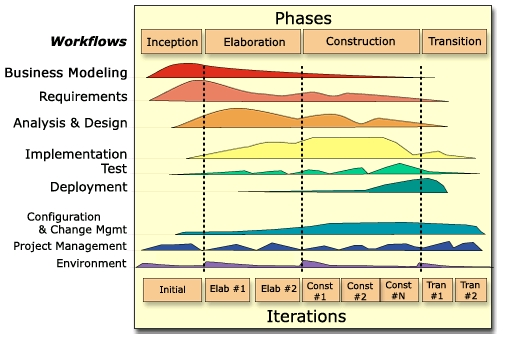
\includegraphics[scale=0.7]{images/rup.jpg}
\caption[Rational Unified process Model]{Illustration of the Rational Unified Process. The waves indicates where the focus and work is taking place in each phase.}
\label{fig:rup}
\end{figure}

\subsection{Scrum}
Scrum is an iterative and incremental development framework for development of complex information systems. When using Scrum, the development of the product is developed in small pieces, with each piece building upon previously created pieces. The use of Scrum requires the team to be divided into specific roles, where each role has its own responsibility. The following are the core roles of the Scrum team\cite{scrum}\cite{sommerville}:
\begin{description}
	\item[Product owner:]{The product owner represents the stakeholders in the project, and is the voice of the customer. It is the product owner's responsibility to ensure that the Scrum team at all times is working with the right things seen from a business perspective.}
	\item[Scrum master:]{The scrum master should act as a buffer between the development team and distracting influences, so that the development team can deliver potentially shippable products at the end of each sprint. The scrum master should keep the development team focused at all times.}
	\item[Development team:]{The development team is made up from three to nine persons with cross-functional skills. This team does all the actual work, including development, testing, designing and so on.}
\end{description}

\subsection{Waterfall model}
The waterfall model is among the first process models to be introduced. In this model, each phase in the development must be completed before one can advance to the next phase. At the end of each phase in the development, a review takes place. In this review it is determined if the project is on the right path and if it should continue or not. The phases in the development do not overlap. \cite{sommerville}

\subsection{Spiral model}
The spiral model is a software development model intended for large and complicated projects. It combines elements from the waterfall model and prototyping models, and uses an iterative approach. Based on this it allows for incremental releases of the product, as prototypes. \cite{sommerville}

%Check if it is written anything about this in the Systemutviklings-bok.
\subsection{Lean software development}
\label{leandev}
Lean is an agile software development methodology that is defined by seven principles\cite{poppendieck}:
\begin{description}
	\item[Eliminate waste.]{Everything that does not add any value to the customer is considered a waste.}
	\item[Amplify learning.]{The development environment should the designed so it amplifies the learning process of the developers. Defects should be prevented by running tests as soon as the code is written.}
	\item[Decide as late as possible.]{By delaying decisions as much as possible, better results can be achieved. There is always uncertainty associated with software development, and delaying options as much as possible results in more flexibility later.}
	\item[Deliver as fast as possible.]{The sooner the product is delivered, the sooner feedback can be received.}
	\item[Empower the team.]{The managers are taught how to listen to the developers, so they can explain better what actions could be taken and give suggestions for improvements.}
	\item[Build integrity.]{The customer needs to have influence and inspection of the project, and an overall experience of the system to be developed.}
	\item[See the whole.]{Decompose the system into smaller parts and find and eliminate defects.}
\end{description}

\section{Existing solutions}
This is a summary of existing solutions similar to the project assignment. This section is divided in two subsections; one for the market application and one for the over-the-air transfer. The existing products were evaluated on the following criteria:
\begin{itemize}
	\item{To what degree the product fits the assignment.}
	\item{Can the product, or parts of it, be reused for the assignment? Can it lead to licensing issues?}
\end{itemize}

\subsection{Market applications}
\paragraph{UbiBazaar} is a prior project which created an universal app store in PHP. This project had potential for serving as a back end, but this was later discarded. The idea of a website for uploading applications was the primary idea for the project. Upon revising the project it was deemed too unstable and incomplete to properly function for our intended use. The project used an outdated version of PHP which caused numerous bugs which would take up too much time to attempt to fix properly.\\

It did have a way for developers to follow each other, which would help creating a community for the developers. For further development of $\mu$CSS, UbiBazaar would also be able to support the development of applications aimed at, for example, Raspberry Pi. This was not included as the goal of our project and therefore discarded.

\paragraph{Google Play} is the market application for Android provided by Google. It is an application that allows for easy browsing and installation of applications on Android devices. It also detects what model of phone that is being used, and only shows applications that are supported by that phone. This functionality is similar to the requirements for the Android application in the project. Since Android users most likely are used to this user interface, shown in figure \ref{googleplay}, it was desirable to emulate this user interface.\\

\begin{figure}[H]
\centering
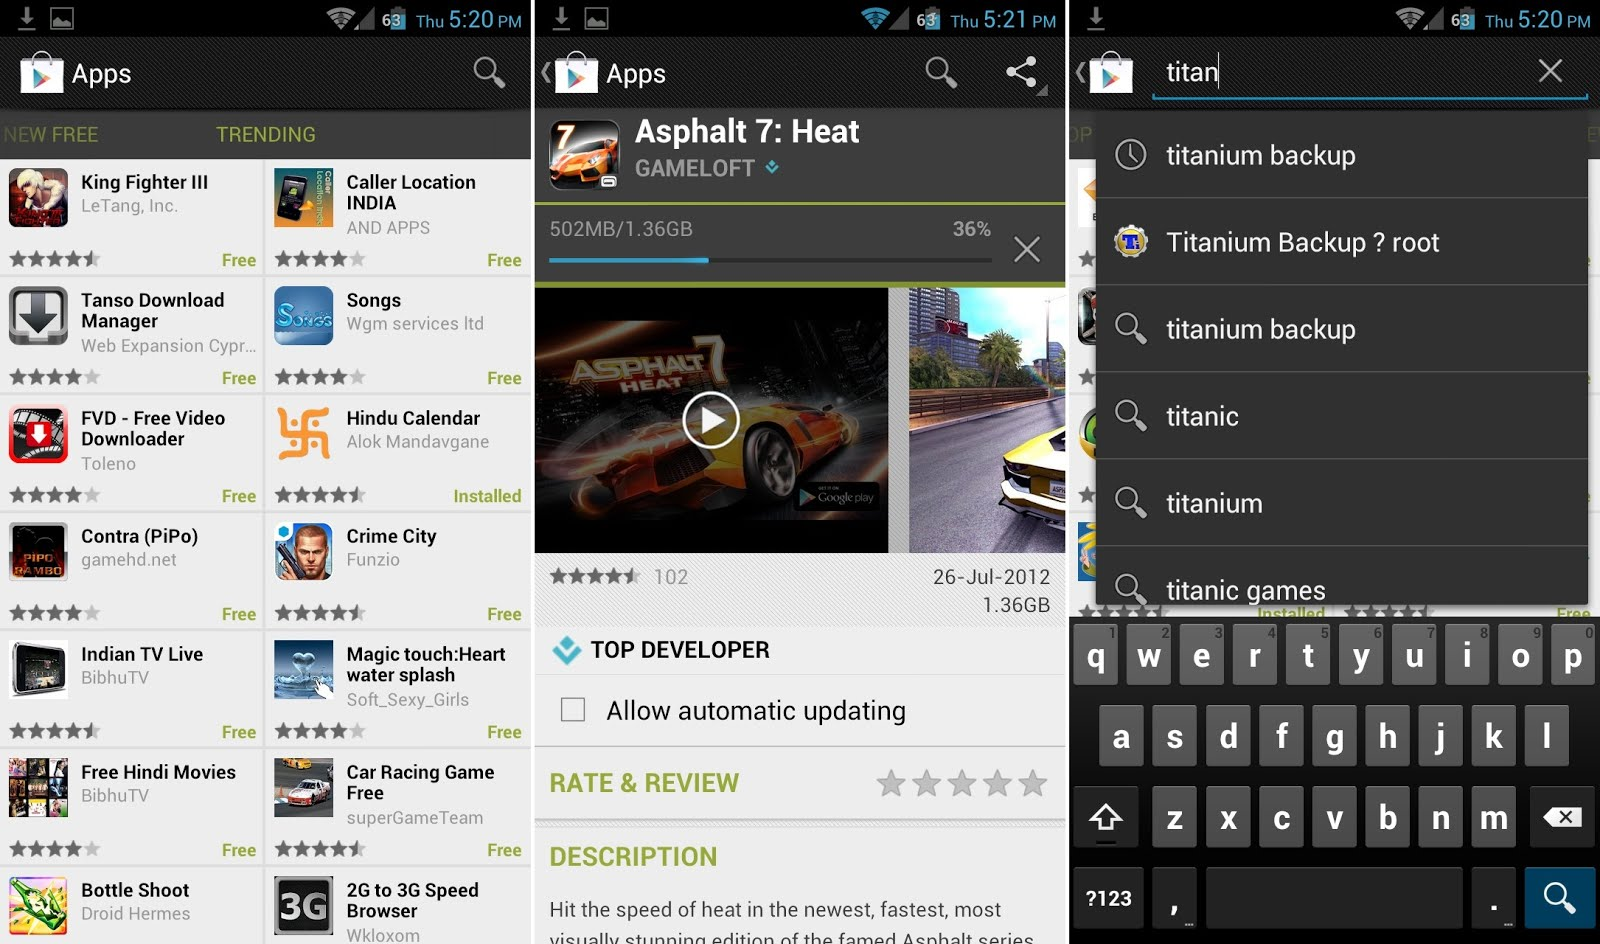
\includegraphics[scale=0.2]{images/Google-Play-Store-APK-3-7-15.jpg}
\caption[Google Play]{Screenshots from the Google Play Store showing their graphical user interface throughout the application.}
\label{fig:googleplay}
\end{figure}

Google Play fits the assignment in the way that is is a market applications where one can download applications. This was useful for the development of the product, since it was possible to use the same principles in the assignment. It was also similar in the way that it was possible to browse for applications on the computer, and ``push'' the application to a mobile telephone. This, however, did not connect via Bluetooth, as the task assignment stated the finished product should. Google Play is not open source and could therefore only be used as a source of inspiration for the project. It was not possible to reuse the code or other parts of the application in the development.



\subsection{Pebble}
Pebble is a watch, shown in figure \ref{pebblewatch}, that offers over the air transfer of applications. The main differences between this watch and a standard Arduino is that Pebble have written a custom operating system in C for this device and contains a Bluetooth connection. Pebble is also using a microcontroller that is significantly faster and contains a lot more memory, which means that it is much easier to develop an operating system for it.\\
\\
To transfer a new application to the watch, the user connects the mobile phone to the watch using Bluetooth. The user can then open the Pebble application store and upload applications made for this watch.

\begin{figure}[H]
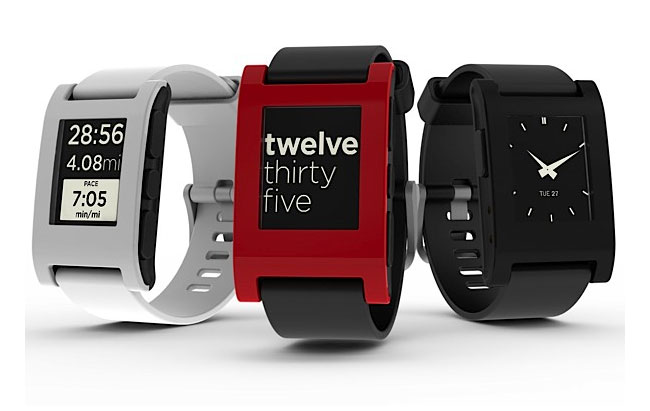
\includegraphics[scale=0.7]{images/Pebble-Smartphone-Watch.jpeg}
\caption[Pebble Watch]{Pebble Watches with different applications changing the watch-faces.}
\label{fig:pebblewatch}
\end{figure}
The principles are quite similar to what we planned to develop, but this platform is not made to expand to other platforms. There was very little documentation on the Pebble website, so the potential for reuse in this project appears minimal.

\section{Over the air transfer}
Usually when you program the Arduino you use a computer with a USB-cable connected to the Arduino board. This is used because it is a stable connection and a standardized cable that everybody has available. This project's main goal was to remove the cable when you are programming the Arduino and move the software over to an Android device. To remove the USB-cable we had to use Bluetooth to communicate between the devices. To connect the Bluetooth to the Arduino it was wired as shown in figure \ref{SimpleArduinoWiring}.
\\
\begin{figure}[H]
\centering
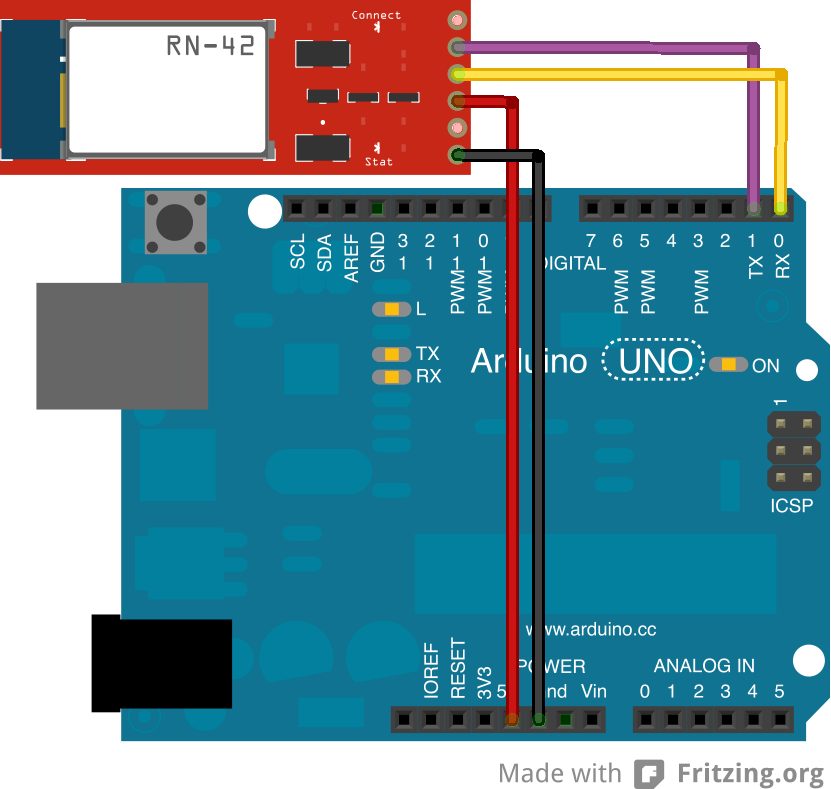
\includegraphics[scale=1.2]{images/wiring_simple.png}
\caption[Wiring Diagram for BT module]{How a Bluetooth piece is connected on an Arduino device.}
\label{fig:SimpleArduinoWiring}
\end{figure}

%TODO ref til RN-42
After a lot of research we made a wireless connection between the Android and the Arduino with a Bluetooth module, with the wiring as shown in figure~\ref{fig:SimpleArduinoWiring}. We used the Bluetooth module RN-42 because it was well documented and easy to connect to the Arduino.\\
\\
The protocol to upload new code to the microcontroller is quite advanced. This must be done without any errors and with the correct baud rate, therefore we rely on the stability of the wireless communication. If an error occurs while uploading the code, it has to start over again.

\chapter{Project management}
The following sections details the project management decisions of the project. This includes choice of development method, team member responsibilities, communication channels and risk analysis.

\section{Development method}
\label{development-method}
Based on the customer requirement of short iterations, it was early decided to adapt an iterative and incremental development method for the project. By working in an iterative manner, it was possible to present prototypes and work done to the customer every week, and at the same time receive feedback. In this fashion it was possible for the customer to continuously present his thoughts on the product, and propose changes where he thought it was necessary. The iterative approach on the project also made it easier for the group to set deadlines and milestones of specific parts of the product.\\
\newline
All the members of the group have taken the course TDT4140 - Systemutvikling, and therefore have some knowledge about different development methods. The Rational Unified Process (RUP) model, as described in Chapter~\ref{prestudy} - Prestudy, is an extensible framework\cite{kruchten} that met the requirements the group had for a process model. RUP was chosen as process model for the project above the other models described in Chapter~\ref{prestudy} as it best met the needs of the group. The fact that the model was tailorable and divided the entire development process into phases that was easy to adapt to made it preferable to the other models examined. It was also appealing that the model required the team to focus on critical risks early in the development to avoid surprises.

\subsection{Changes to description}
As mentioned above, it was clear that the use of an iterative model was in order. The specific documentation of the development method was deferred for three weeks, however. This was due to the uncertain future of the project (over the air installation was said to potentially be impossible) and the need to get the first iteration presented to the customer; precisely documenting the development method was deemed to be wasteful at that point in time. The development method description was also refined between the preliminary version and the midterm version of the report.\\
\newline
It was decided to adopt RUP as process model, though with some minor changes. First of all, the Transition phase of the model was deemed unnecessary. This was mainly due to the lack of time and resources for beta testing and new versions of the product. This phase was instead replaced by the closeout phase, described in chapter~\ref{projectplanning}. Further, no cost estimates were developed for the project. Because no money were involved in the production of the product, this was also deemed unnecessary. Time and resource estimates, however, were established during the Inception phase. \\
\newline
In addition to the changes mentioned above, use of Lean principles was adapted from the start of the project. As described in the section about Lean Software Development, this methodology is defined by seven principles. Of these, especially \emph{Eliminate waste} and \emph{Build integrity} were used actively by the team during the development of the product and project report. These principles is described in chapter~\ref{leandev}.

\section{Team roles}
The group was organized in different roles based on skill and experience. Each team member was given a responsibility for some code-packages. Further, the team was divided into six subgroups where each member was held responsible for his or her group. These groups was respectively: group leader, documentation and substitute leader, Android and GUI, Arduino$\texttrademark$ and PUI, over the air and test.
The distribution of team roles are listed in Table~\ref{table:teamroles}

\subsection{Role description}
The division of the group was an important feature. Every member knew who to contact about a specific problem or task.\\

\begin{description}
	\item[Group leader]{was responsible for the progress in the overall project. This person ensured progress and priorities for deadlines.}
	\item[Documentation and substitute leader]{was responsible for management of documentation and reports. In absence of the group leader, this person took on the group leader's responsibilities. This person was also responsible for contact with the customer and supervisor.}
	\item[Android and GUI developer]{was responsible for the Android development of the project.}
	\item[Arduino$\texttrademark$ and PUI developer]{was responsible for the Arduino$\texttrademark$ part of the project. This implies contacting the Arduino$\texttrademark$-lab, requisitions for hardware, the coding part and over-the-air installation. This role was also responsible for development of the PUI examples.}
	\item[Over the air developer]{was responsible for programming the Arduino$\texttrademark$ over the air. This person was also responsible for making the first prototype with a Bluetooth$\textsuperscript{\textregistered}$  connection.}
	\item[Test developer]{was responsible for developing and executing tests for the complete project.}
\end{description}

\begin{table}[H]
\captionof{table}{Roles}
\centering
\label{table:teamroles}
\begin{tabular}{|l|l|}
\hline
	{\bf Name} & {\bf Role}\\
\hline
	Jeppe Benterud Eriksen & Group leader\\
\hline
	Nina Margrethe Smørsgård & Documentation and substitute leader\\
\hline
	Robin Tordly & Android and GUI developer\\
\hline
	Bjørn Arve Fossum & Arduino$\texttrademark$ and PUI developer\\
\hline
	Ståle Semb Hauknes & Over the air developer\\
\hline
	Wilhelm Walberg Schive & Test developer\\
\hline
\end{tabular}
\end{table}

\subsection{Division of labor}
The division of labor between the members of the group was largely done through the use of issues on GitHub (chapter \ref{sec:GitHub}). On this site, whenever a task arose, it was created as an issue. This way, all the members could see what needed to be done, assign different issues to themselves, see what others were working on and therefore choose an appropriate issue to start working on.

Throughout the project the main consensus of the group has been to meet every day as long as there is not something else interfering. This has caused the group to work together almost every day and thus if a problem was met it could be dealt with quickly. Usually these meeting started at 09:00-10:00 and ended around 16:00. Any and all work done by anyone was registered in a document to ensure correct activity plans.

\section{Communication}
Most of the communication within the group was done at group meetings and when the group was working together. For communication between group members outside the meetings it was decided that the group should only use email and Skype. This was decided to avoid the confusion that might arise from using numerous channels of communication. Mobile phone was also used when immediate contact was necessary.\\
\newline
% What about GitHub?
Communication between the group and the customer was mainly done in meetings or by email. The same applies for communication with the supervisor.

\section{Project planning}

\label{projectplanning}

In this section the planning of the project will be presented. The project was divided into five large milestones to represent the different phases of the project. The phases of the Rational Unified Process (RUP) is not explicitly stated in the work breakdown structure, as some of the milestones stretches over several of the phases in the process model. \\
\newline
In the work breakdown structure (WBS), the first part of the Project Management activity and the Planning activity represents the inception and elaboration phase of RUP. Further, the Execution and Testing activities represents the construction phase. As mentioned above the transition phase of RUP was deemed unnecessary. It was expected that tasks related to project management would appear at least until the technical part of the project was concluded, and it was therefore decided to let this activity run through the larger part of the project. In the closeout phase work on the final report was to be prioritized.

\subsection{Work breakdown structure (WBS)}
The WBS is a view on what work packages the project encompasses. It helps with communicating the work and processes to easily execute the project. The duration-time show how much estimated time one task requires, and gives an assessment on how much effort is needed to complete the task.

\subsubsection{Gantt chart}
Gantt chart showing the initial work breakdown structure created in the project.
\begin{figure}[H]
\makebox[\textwidth][c]{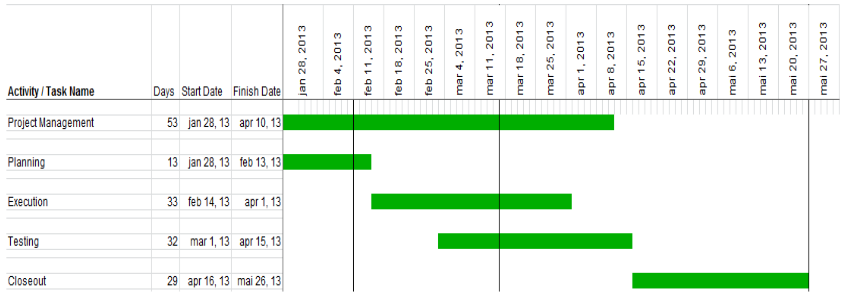
\includegraphics[width=1.2\textwidth]{images/gantt-diagram.png}}
\caption{Gantt chart. Milestones are marked using vertical lines}
\end{figure}

\subsubsection{Work breakdown structure table (WBS table)}
Table~\ref{fig:wbstable} is showing a detailed overview of all the tasks to be preformed in each of the milestones. The WBS code of each task is used to relate it to the WBS tree shown below. This table also contains a description of each task.

\begin{longtable}{|m{0.1 \textwidth}|m{0.1 \textwidth}|m{0.2 \textwidth}|m{0.35\textwidth}|m{0.15 \textwidth}|}
\hline
	\rowcolor{Gray}
	\textbf{Level} & \textbf{WBS{ }Code} & \textbf{Element name} & \textbf{Definition} & \textbf{Duration}\\
	\endfirsthead% 
	\multicolumn{5}{l}%
	{{\bfseries Continued from previous page}} \\ \hline
	\rowcolor{Gray}
	\textbf{Level} & \textbf{WBS{ }Code} & \textbf{Element name} & \textbf{Definition} & \textbf{Duration}\\
\hline
	\endhead%
	\hline
 
	\hline \multicolumn{5}{|l|}{{Continued on next page}} \\ \hline
	\endfoot%
 
	\endlastfoot%

	1 & 1 & $\mu$C Software Store & All work to implement an application store for Arduinos and over the air innstallation with two example PUIs & \\
\hline
	2 & 1.1 & Project management & The work to initiate the project and distribute responsibilities & \\
\hline
	3 & 1.1.1 & Meetings with customer & Determine the project status and decide on requirements & \\
	 & 1.1.2 & Demonstration and play for the customer of the team's understanding of the requirements & Project team evaluates and proposes recommendations & \\
\hline
	 & 1.1.3 & Risk management & Creating risk analysis and agreements within the group and the project & \\
\hline
	 & 1.1.4 & Status report & Write the status report & \\
\hline
	2 & 1.2 & Planning & & \\
\hline
	3 & 1.2.1 & Requirements specification & & \\
\hline
	 & 1.2.2 & Determine Project team & Give each menber a role and distribute tasks & \\
\hline
	 & 1.2.3 & Supervisor meeting & Meeting wih supervisor for instruction and guidance & \\
\hline
	 & 1.2.4 & Develop project plan and use cases & & \\
\hline
	 & 1.2.5 & Research & & \\
\hline
	 & 1.2.5.1 & Research on over the air innstallation & Do research on bluetooth installation on arduinos & \\
\hline
	 & 1.2.5.2 & Research UbiCollab libraries & & \\
\hline
	2 & 1.3 & Execution & Programming and execution of the project & \\
\hline
	3 & 1.3.1 & Project kickoff meeting & First meeting with customer to evaluate knowledge and agree on further meetings & \\
\hline
	 & 1.3.2 & Verify \& validate user requirements & Determine whether the group is in tune with the customers vision of the project requirements & \\
\hline
	 & 1.3.3 & Design system & & \\
\hline	  
	 & 1.3.4 & & & \\
\hline
	 & 1.3.5 & Produce Software & & \\
\hline
	 & 1.3.6 & Instalation over the air implementation & & \\
\hline
	 & 1.3.7 & Documentation & & \\
\hline
	2 & 1.4 & Testing & & \\
\hline
	3 & 1.4.1 & Develop unit tests & & \\
\hline
	 & 1.4.2 & User testing & & \\
\hline
	 & 1.4.3 & Stress testing & & \\
\hline
	 & 1.4.4 & System Testing & & \\
\hline
	2 & 1.5 & Closeout & & \\
\hline
	3 & 1.5.1 & Creating final project report & & \\
\hline
	 & 1.5.2 & Delivery to customer & & \\
\hline
\end{longtable}
\captionof{table}{Work Breakdown Structure}


\subsubsection{Work breakdown structure tree (WBS tree)}
This is the WBS tree made for this specific project.
\begin{figure}[H]
\vspace*{-1.5in}
\hspace*{-1.2in}
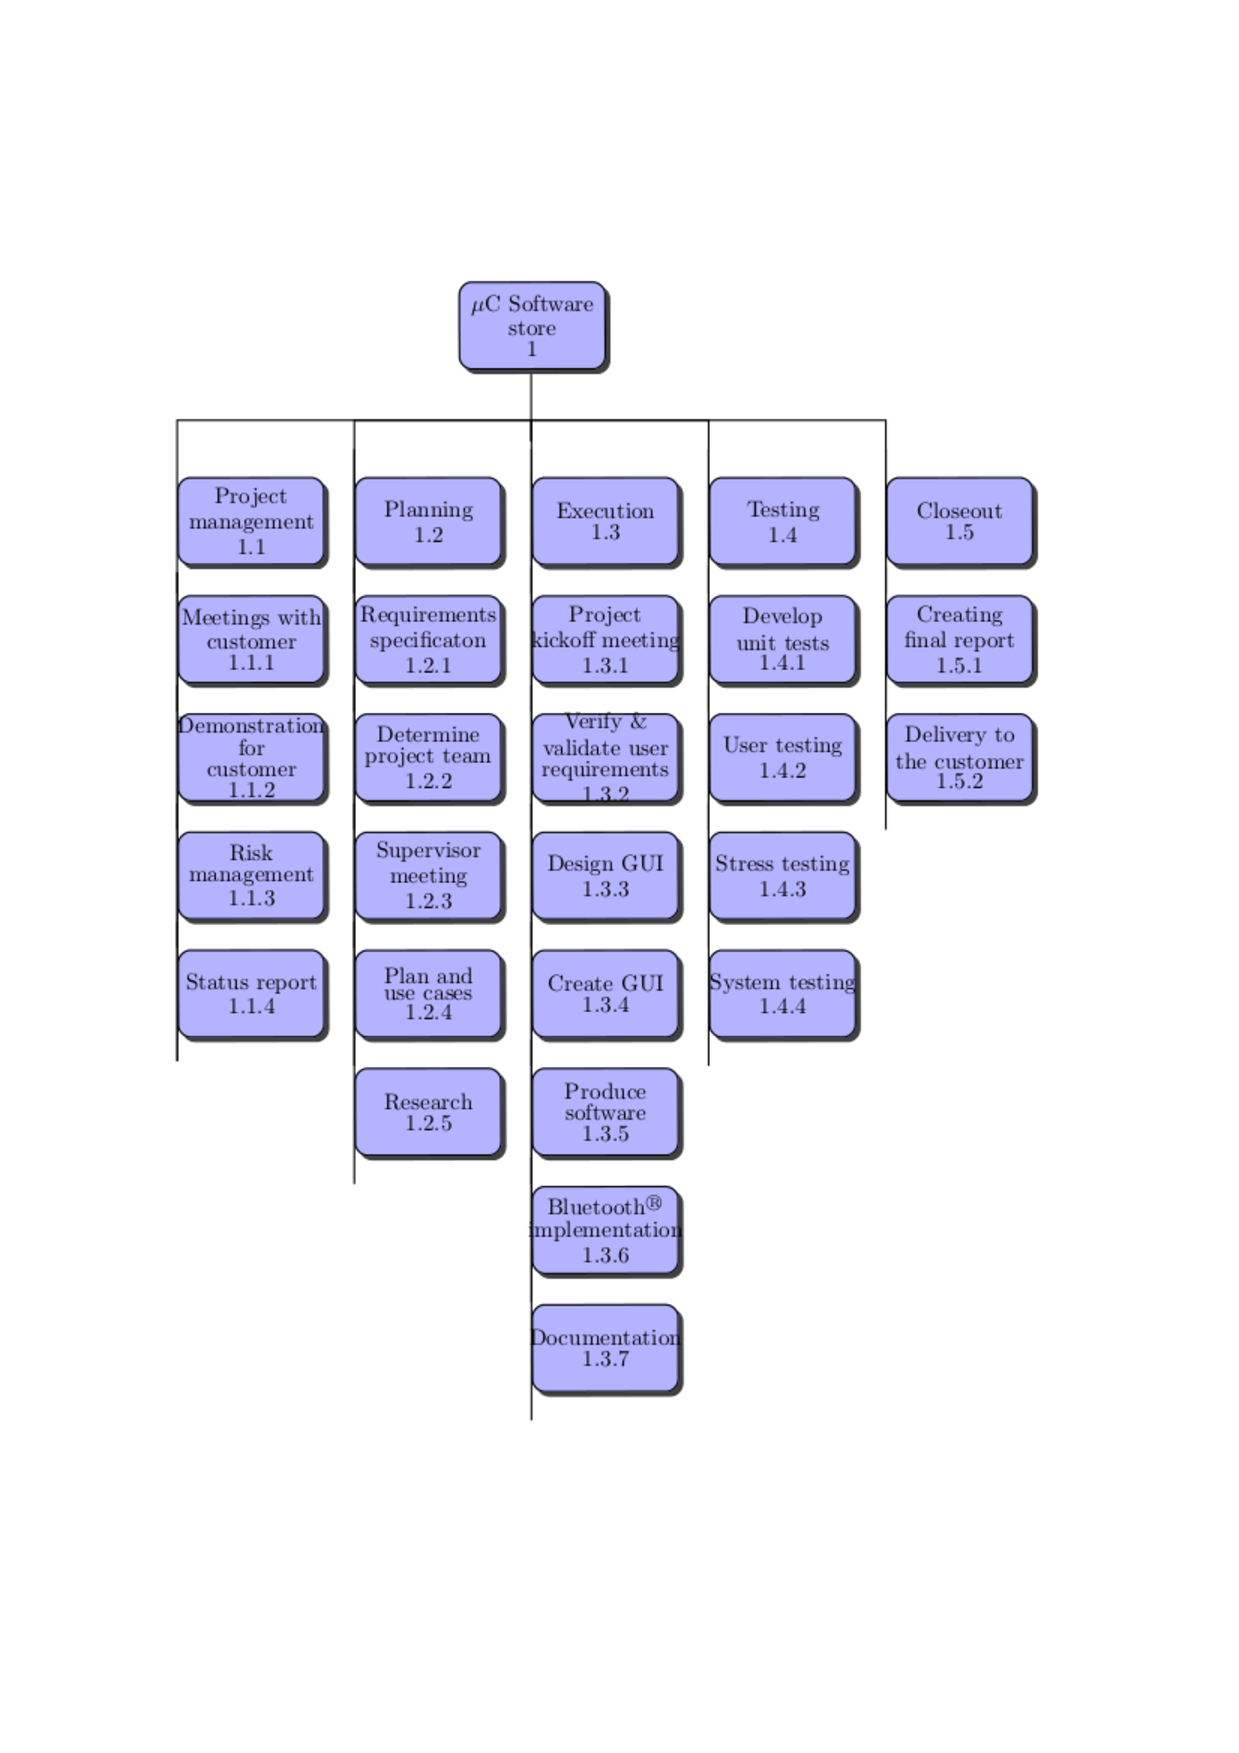
\includegraphics[trim=0cm 4cm 0cm 0cm]{figures/wbs-tree2.pdf}
\captionof{figure}{WBS tree showing a more detailed overview of the different tasks in each of the five milestones.}
\end{figure}

\subsection{Editions to WBS}
Due to challenges and unexpected work that emerged during the project, it was not possible to follow the WBS completely. First of all, a lot of unplanned work arose in connection with the implementation of STK500 in Java. The result of this was that not all group members were able to move to the closeout phase at the same time, as there still was unfinished work on the protocol.

\section{Risk analysis}
The risk analysis as shown in table~\ref{fig:risktable} states risks identified by the team. The importance of a risk is calculated by multiplying likelihood and impact. Higher number means higher importance for the project.
\captionof{table}{Risk analysis}
\label{fig:risktable}
\begin{longtable}{|m{0.15 \textwidth}|m{0.1 \textwidth}|m{0.1 \textwidth}|m{0.1 \textwidth}|m{0.185 \textwidth}|m{0.185 \textwidth}|}
\hline
	\rowcolor{Gray}
	\textbf{Description} & \textbf{Likeli{-}hood} & \textbf{Impact} & \textbf{Impor{-}tance} & \textbf{Preventive\newline Action} & \textbf{Remedial\newline Action}\\
	\endfirsthead%
	\multicolumn{6}{l}%
	{{\bfseries Continued from previous page}} \\ \hline
	\rowcolor{Gray}
	\textbf{Description} & \textbf{Likeli{-}hood} & \textbf{Impact} & \textbf{Impor{-}tance} & \textbf{Preventive\newline Action} & \textbf{Remedial\newline Action}\\
\hline
	\endhead%
	\hline

	\hline \multicolumn{6}{|l|}{{Continued on next page}} \\ \hline
	\endfoot%

	\endlastfoot%

	Illness & 7 & 2 & 14 & Good\newline communication and effective use of GitHub & Increase workhours and exchange tasks and\newline responsibilities\\
\hline
	Project\newline complexity & 6 & 5 & 30 & Don't take on too much work & Cut down the demands\\
\hline
	Customer\newline issues & 1 & 5 & 5 & Agreement with customer and weekly feedback from customer & Use the\newline original\newline requirement specification\\
\hline
	License\newline incompability & 7 & 7 & 49 & Avoid\newline integrating components with incopatible licenses & Discover other implementations or implment from scratch\\
\hline
	Group\newline conflicts or disagreements & 3 & 3 & 9 & Keep close\newline contact to avoid\newline surprises.\newline Leader takes\newline action & Contact\newline supervisor and make an\newline appointment\\
\hline
	Over the air complexity & 8 & 8 & 64 & Have multiple\newline alternative\newline solutions and keep close\newline contact with customer & Detail what was attempted as well as why it couldn't be solved in the final report.\\
\hline
	Personal matters & 8 & 5 & 40 & Not much\newline preventative action can be taken & Keep in touch and stay\newline updated. In case you still can do tasks, claim one and tell the\newline others\\
\hline
\end{longtable}

\chapter{Requirements}
This chapter describes the functional and non-functional requirements of the system, together with use cases. At the end of the chapter the changes in requirements during the project will be described.
The requirements of the project will be kept high level and vague, to facilitate making choices as late as possible.
\section{Functional requirements}
	\begin{table}[H]
	\begin{tabularx}{\linewidth}{lX}
		\textbf{FR01} & \textbf{Over the air installation}\\
 		& The Android application and the Arduino device should communicate over Bluetooth$\textsuperscript{\textregistered}$  and install an arbitrary application from the Arduino Store in a simple two step process.\\
		\textbf{FR02} & \textbf{Easy to use interface}\\
 & The Arduino Store application should be easy to use and easy to understand. It should not be necessary to do anything on the Arduino except for starting it. On startup it should search for nearby Bluetooth$\textsuperscript{\textregistered}$  connections with paired devices.\\
 		\textbf{FR03} & \textbf{Example PUIs}\\
 & To demonstrate the Arduino Store (on Android), over the air installation, and the application in action on an Arduino.\\
		\textbf{FR04} & \textbf{Validation of Arduino hardware and software}\\
 & The Android application should by default hide Arduino applications in the Arduino Store which are incompatible with the Arduino device depending on memory requirements and connected devices.\\
	\end{tabularx}
		\caption{Functional Requirements}
	\end{table}

\section{Non-functional requirements}
	\begin{table}[H]
	\begin{tabularx}{\linewidth}{lX}
		\textbf{NFR01} & \textbf{Usability}\\
		 & Both old and young persons should be able to understand how to use the application and install arduino-apps.\\
		\textbf{NFR02} & \textbf{Reliability}\\
		 & The application on the Arduino should work and start if rebooted.\\
		\textbf{NFR03} & \textbf{Open source}\\
		 & The project is under European R\&D project SOCIETIES. All source code will be open source under Apache 2.0 license.\\
		\textbf{NFR04} & \textbf{Platform compability}\\
		 & Arduino Store should be compatible in Android 2.3 and newer. See FR04 for compatibility for Arduinos.\\
		\textbf{NFR05} & \textbf{Extensibility}\\
		 & It should be easy to add features and extend this product later. The system should therefore be modular to simplify further development.\\
	\end{tabularx}
		\caption{Non-functional requirements}
	\end{table}

%TODO: Do the latex stuffs so it looks nice.
%TODO: bestemme requirements som skal forsvinne og legges til

\section{Use-Cases}
\begin{figure}[H]
\centering
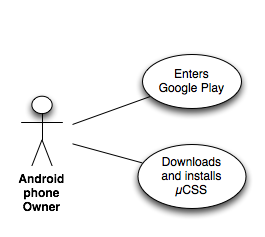
\includegraphics[scale=0.7]{images/UseCase1}
\caption{Use case 1}
\end{figure}

    \begin{table}[H]
        \begin{tabularx}\linewidth{ |m{0.3 \textwidth} |X|   }
            \hline
                ID           & 1 \\
            \hline
                Name             & Install $\mu$CSS \\
            \hline
                Goal             & Have $\mu$CSS installed on the Android device\\
            \hline
                Actors           & Android device owner\\
            \hline
                Prequisite       & The actor have a Android device with Google Play\\
            \hline
                Main Flow        &  1. Opens Google Play \\
                                 &  2. Search for ''$\mu$C Software Store'' \\
                                 &  3. Installs the application \\
            \hline
                Alternative Flow & None\\
            \hline
                Parent UC        & None\\
            \hline
                Child UC         & All\\
            \hline
        \end{tabularx}
        \caption{Use case 1}
    \end{table}

\begin{figure}[H]
\centering
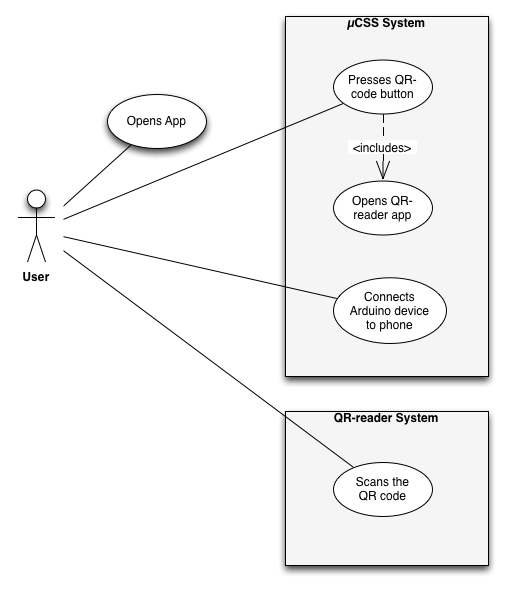
\includegraphics[scale=0.7]{images/UseCase2}
\caption{Use case 2}
\end{figure}

\begin{table}[H]
    \begin{tabularx}\linewidth{ |m{0.3 \textwidth} |X| }
        \hline
            ID               & 2 \\
        \hline
            Name             & Pair Arduino device and Android device with QR code\\
        \hline
            Goal             & Connect the Arduino device to the Android application with the use of QR code\\
        \hline
            Actors           & Arduino device owner\\
        \hline
            Prerequisite     & Installed $\mu$CSS \\
                             & Installed predefined QR-reader\\
        \hline
            End requirement  & The Arduino device is connected to the phone via Bluetooth$\textsuperscript{\textregistered}$ \\
        \hline
            Main flow        &  1. User opens $\mu$CSS \\
                             &  2. User presses the button indicating that he wants to pair with the Arduino device using QR code \\
                             &  3. The system opens the QR reader application \\
                             &  4. The QR reader application reads the QR code and returns the information it contains\\
                             &  5. The system pairs with the Arduino device \\
        \hline
            Alternative flow &  3.a. The user does not have the right QR code reader installed \\
                             &  3.b. The system prompts the user if he wants to install the QR code reader \\
                             &  3.c. If no: stop \\
                             &  4.a. The QR reader is unable to read the QR code \\
                             &  4.b. Try again or stop\\
        \hline
            Parent UC        & 1\\
        \hline
            Child UC         & 7\\
        \hline
    \end{tabularx}
    \caption{Use case 2}
\end{table}

\begin{figure}[H]
\centering
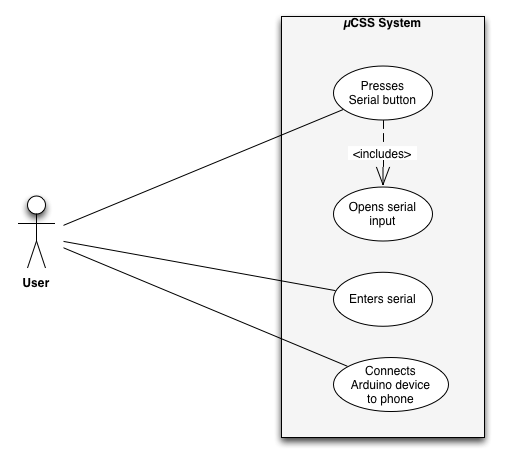
\includegraphics[scale=0.7]{images/UseCase3}
\caption{Use case 3}
\end{figure}

\begin{table}[H]
    \begin{tabularx}\linewidth{ |m{0.3 \textwidth} |X| }
        \hline
            ID               & 3 \\
        \hline
            Name             & Pair Arduino device with Android device using serial \\
        \hline
            Goal             & Connect the Arduino device to the Android application with the use of QR code \\
        \hline
            Actors           & Arduino device owner \\
        \hline
            Prerequisite     & Installed $\mu$CSS \\
                             & Intstalled predefined QR-reader \\
        \hline
            End requirement  & The Arduino device is connected to the phone via Bluetooth$\textsuperscript{\textregistered}$ \\
        \hline
            Main flow        &  1. User opens $\mu$CSS \\
                             &  2. User presses the button indicating that he
                                    wants to pair with the Arduino device using a serial code \\
                             &  3. System opens dialog box for input\\
                             &  4. The user types the serial \\
                             &  5. The system pairs with the Arduino device \\
        \hline
            Alternative flow &  4.a. The user misspells the serial \\
                             &  4.b. The system displays an error, and prompts again \\
        \hline
            Parent UC        & 1 \\
        \hline
            Child UC         & 7 \\
        \hline
    \end{tabularx}
    \caption{Use case 3}
\end{table}

\begin{figure}[H]
\centering
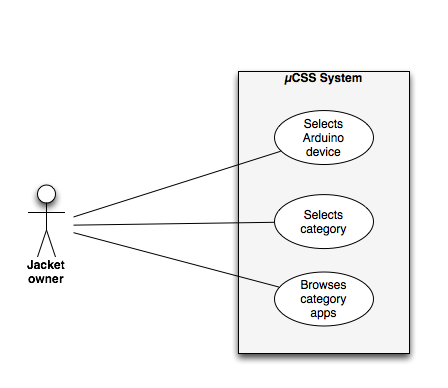
\includegraphics[scale=0.7]{images/UseCase4}
\caption{Use case 4}
\end{figure}

        \begin{table}[H]
        \begin{tabularx}\linewidth{ |m{0.3 \textwidth} |X| }
            \hline
                ID               & 4 \\
            \hline
                Name             & Browse apps \\
            \hline
                Actors           & Arduino device owner \\
            \hline
                Prequisite       & Installed $\mu$CSS \\
            \hline
                End Requirement  & None \\
            \hline
                Main Flow        &  1. The user opens $\mu$CSS \\
                                 &  2. The user selects the an Arduino device \\
                                 &  3. The user selects category (One category is named ''all'') \\
                                 &  4. The user browses apps \\
            \hline
             Alternative Flow    & 2.a. The user does not select Arduino device, but browses anyway \\
           \hline
        \end{tabularx}
        \caption{Use case 4}
    \end{table}



\begin{figure}[H]
\centering
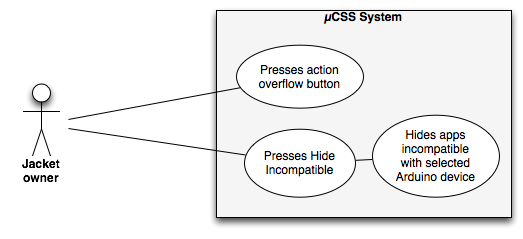
\includegraphics[scale=0.7]{images/UseCase5}
\caption{Use case 5}
\end{figure}



\begin{figure}[H]
\centering
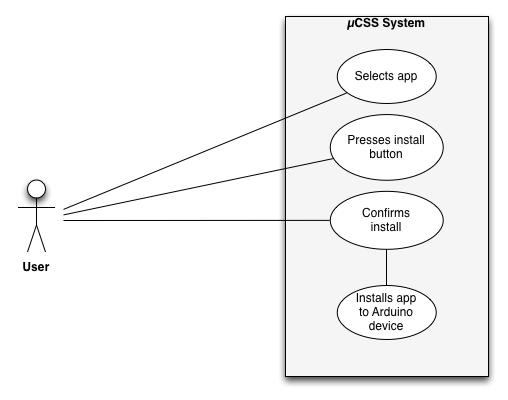
\includegraphics[scale=0.7]{images/UseCase6}
\caption{Use case 6}
\end{figure}

\begin{table}[H]
    \begin{tabularx}\linewidth{ |m{0.3 \textwidth} |X| }
        \hline
            ID               & 6 \\
        \hline
            Name             & Install application on Arduino device \\
        \hline
            Goal             & Connect the Arduino device to the Android application with the use of QR code \\
        \hline
            Actors           & Arduino device owner \\
        \hline
            Prerequisite     &  Installed $\mu$CSS \\
                             &  Arduino device connected to $\mu$CSS \\
        \hline
            End requirement  & The application is installed on the Arduino device \\
        \hline
            Main flow        &  The user selects the desired application \\
                             &  The user presses the ''install'' button \\
                             &  The user confirms the installation \\
                             &  The application is installed at the Arduino device \\
        \hline
            Alternative flow & none \\
        \hline
            Parent UC        & 1, 2, 3, 4, 5 \\
        \hline
            Child UC         & none \\
        \hline
    \end{tabularx}
    \caption{Use case 6}
\end{table}


\section{Changes in requirements after midterm}
Approaching midterm it was discovered that the over the air transfer of PUI apps to an Arduino device proved to be more demanding than planned. After an extraordinary meeting with the customer it was decided to change the focus of the assignment. \\
\newline
The goal of the project remained consistent with previous statements. A prototype of the Android store application had been made, though not all functionality was implemented and tested. Further work on the Android application were temporarily put on halt. At this point the resources were primarily focused on implementing the STK500 protocol in Java to allow for programming of Arduino from an Android device. Se below for concrete additions and removals on the requirements.

% Add more as needed
\subsection{Additions}
\paragraph{STK500 protocol} As mentioned above, implementing the STK500 protocol proved more demanding than expected. Initial research done by the group on this area showed that an Java implementation of AVRDude already existed. Further research on the implementation, however, showed that it could not be used as it required programs not available on Android to be installed on the device. As of midterm, implementing the STK500 protocol in Java were added to the requirements.

\subsection{Removals}
\paragraph{$\mu$CSS server component} In agreement with the customer it was decided to remove the server side component of the assignment from the requirements. This was decided to pool resources to other more critical tasks.

\paragraph{Sync adapter} As the server component of the assignment was removed from the requirements, there was no need for the sync adapter.


\chapter{Development environment}
In this chapter the different tools and resources used in relation with the project will be presented. The general requirement for a tool to be used is that it is multi-platform, as three different operating systems is in use within the group. It is also preferable that the tool is free, since this is a project that does not generate income.

\section{Development tools}
These are tools used in the development of the project. They have contributed in the technical aspects of development such as coding.
\subsection{Integrated Development Environments (IDEs)}
An IDE is used by programmers to develop and program applications. These are the IDEs that was used during the project.

\subsubsection{Eclipse}
Eclipse is a freely available IDE implemented in Java. It has extensive plugin support and anyone can publish a plugin to support another programming language, versioning software or new program features altogether. Eclipse provides useful, time saving functionality to developers, such as an extensive live debugging suite in addition to checking code syntax and providing auto completion of method calls.\\
\newline
Eclipse was chosen for Android development, due to previous experience with the software and good plugin support for targeting different versions of the Android API. Using a plugin for Arduino support was also considered, but the functionality of the available plugin was found lacking. %Ståle, kan du si mer her?

\paragraph{Mylyn}
is a plugin meant to integrate with other plugins that provide access to task, issue and bug tracking repositories. Issues can be referenced or created quickly from the Eclipse IDE while coding, and the plugin can be configure to show relevant code sections when selecting an issue to work on. The group used a GitHub connector for Mylyn to get Mylyn to display and work with GitHub issues.

\paragraph{The Android Software Development Kit (SDK)}
provides access to several versions of the Android API through the use of an installation manager. This allows for simple updating when new versions of the API are released, as well as supporting older devices. A simulator for testing against different Android devices is also available.

\subsubsection{Arduino IDE}
The Arduino IDE is provided by the creators of the Arduino platform as a free and open source program. It provides syntax checking, example programs, as well as basic editing tools. The IDE handles compilation of Arduino code into C and C++ code the regular microcontroller tools can handle (the IDE includes and depends on tools developed by Atmel, the company behind the chip Arduino uses) and can pass it on to an integrated uploading tool (avr-dude) to get it running on the Arduino.\\
\newline
The official Arduino IDE was considered for coding the Arduino component in, but due to its limited text and code related feature set (lacking features such as auto complete), the IDE was not used for coding.

\subsection{Codebase management and versioning}
The tools described in this section is used for versioning and managing the codebase. 

\subsubsection{Git Version Control Software}
Git is a free, open source Version Control Software (VCS) with support for both local and remote repositories. It keeps track of differences between versions of files and allows for offline commits and branch creation, as this is done locally first before pushing the updates to a repository.\\
\newline
There are various terminal and front-end solutions available, including a GUI version from GitHub and Eclipse plugins. Past experiences with Git plugins for Eclipse led to a decision to use terminal software, as the GitHub program lacked advanced functionality regarding branching, among others. Another benefit with that solution was that the VCS then was IDE- and platform-independent and that there was no need to use the IDE for working with the report repository.

\subsubsection{GitHub}
\label{GitHub}
GitHub hosts repositories for use with the Git VCS. They also provide basic issue tracking and social features, such as following other developers or projects. Paying customers can elect to hide their code, while free users have to share their code with everyone (one user can however keep one hidden project as long as he is the sole developer). The customer required source code to be uploaded to GitHub and also recommended use of GitHub for requesting assistance using issues - a recommendation that was followed.

\section{Project management tools}
The tools mentioned here are tools used in general management of the project. This includes elements such as the planning of meetings, writing and sharing information between group members.

\subsection{Google Docs}
Google Docs is a free to use online office suite that allows users to simultaneously edit documents of different types (text, spreadsheet, presentation, et cetera), which was of great use when the group was working together on documents. It also supports document chat and comments (temporary chat/forum thread-like structure). Google Docs was used for editing the preliminary version of the report and other documents concerning the project.

\subsection{Microsoft Word}
Microsoft Word is the de facto standard Word Processor, with support for many different effects (blinking letters, 3D text and so on). Content creation and formatting tasks are nearly completely intertwined, making it tricky to maintain a consistent document as the documents grow larger. Microsoft Word was used to generate certain graphs for the preliminary reports.

\subsection{\LaTeX}
\LaTeX ~is a macro-improved version of Tex used for typesetting documents. It is free and open source. The general idea is to separate content creation and formatting to create consistent documents effectively without being distracted by the appearance of the content. After the preliminary report, work on the report was written in \LaTeX.

\subsection{Google Calendar}
Google Calendar is a free to use online calendar. It supports both private and public events. Google Calendar allows for simple calendar synchronization across different devices and platforms. A shared calendar in Google Calendar was created to make it easier to keep track of group meetings, meetings with the customer and so on.

\subsection{Dropbox}
Dropbox is a cross platform file synchronization and sharing service. Files in a specified folder are automatically kept in sync among different devices. It is also possible to share folders with other users and with the world at large (this will also serve HTML pages). The basic service is free, but comes with limited storage space. Dropbox was used for sharing of various files within the group, such as compiled versions of the report, data sheets for Arduino components and so on.

\subsection{TextMate and Sublime Text 2}
These tools is sophisticated text editors that can be used for coding, markup and regular text editing. In the project they were used for editing of the report and coding for Arduino. While TextMate is for OS X only, Sublime Text is cross-platform.

\subsection{Wunderlist}
Wunderlist is a free todo list tool supporting shared lists. It supports sharing tasks between the participants of a to-do list with reminders and notes. Wunderlist was used to serve reminders for other, non-coding related tasks, like scheduling meetings or booking rooms.

\subsection{Doodle}
Doodle is a free online tool for scheduling events. It allows a user to create an event and aims to simplify scheduling of events by ''polling'' the participants when they are available. When the participants of the event have answered, one can easily view when all participants are available for meeting. Doodle was used to schedule the first meetings the group had, before regular meetings were established.

\subsection{Fritzing}
Fritzing is a tool that lets you draw circuit boards and wiring diagrams. This makes simple diagrams that are easy to understand and easy to reproduce for users that do not understand electronics. Often used with the Arduino platform because usually the users of this platform have no electronic experience. Most of the standard electronic equipment used with the Arduino are included in this tool. Fritzing was used to create the wiring diagram of the Bluetooth$\textsuperscript{\textregistered}$ wiring and the iJacket clone.

\subsection{OmniGraffle}
OmniGraffle is a software used to draw diagrams and charts. This program makes it easy to draw neat diagrams and charts without spending much time on this. OmniGraffle was used to create ER-diagram and use cases.

\section{Test Management}
The tools mentioned here were used for preparation and creation of tests for the project. 

\subsection{Robotium}
Robotium is a JUnit based framework for the creation of automatic unit testing in Android. It automates the created tests by going through the Android application as described in the tests. This shows the tester what is done and even though it may be slow it allows the tester to see if a mishap is due to the test itself being wrong, for example being in the wrong screen.

\chapter{Design and implementation}
In this chapter the design and system architecture of the product will be presented. The reader will learn about how the different components of the product are put together, and how the design of the application was planned.

\section{System architecture}
	The design was divided into several modules:
	\begin{itemize}
		\item{Bluetooth connection between the Android and the Arduino}
		\item{Synchronization with the local SQLite database}
		\item{Android application view (the visible design)}
		\item{A service that contains the protocol for installing over-the-air}
	\end{itemize}
	\vspace{0.2in}
	
	The system design was implemented such that further developing and extension should be as modular and easy as possible.
	Therefore it was designed as a plugin-like system where you easily can implement your own protocols against a desired device, e.g. Raspberry Pi. The application only supports the STK500v1 protocol and therefore only connections towards Arduino devices (and with some work other STK500 based devices). The design for the connection to other devices was done as shown in Figure~\ref{fig:btconnection_service_stk500}.\\

	\begin{figure}[H]
	\centering
	\hspace*{-0.75in}
	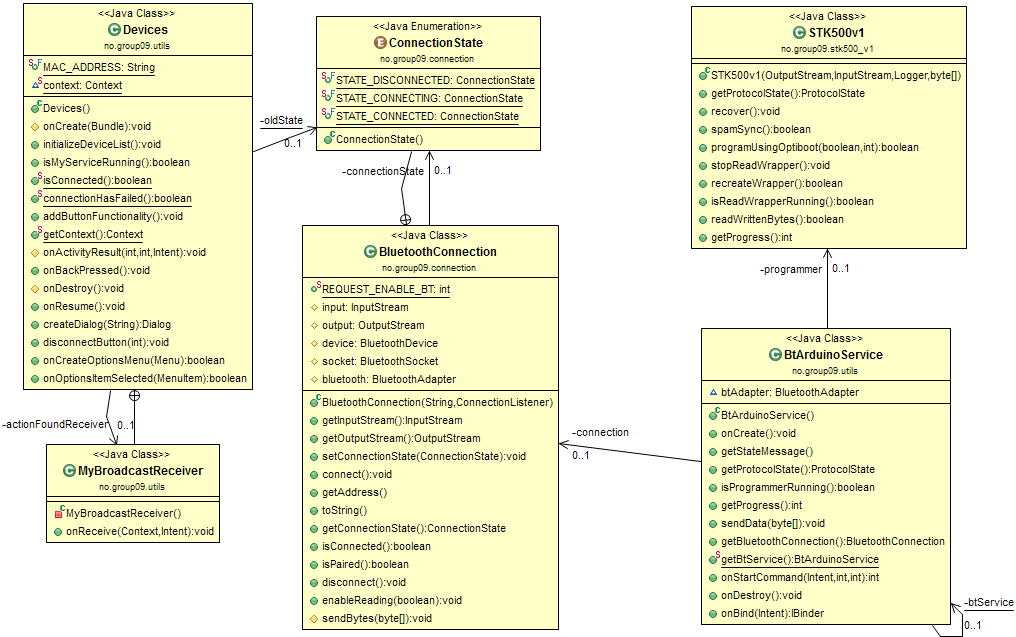
\includegraphics[scale=0.85]{images/UML/btconnection_service_stk500.png}
	\caption[BT connection in service]{The Bluetooth connection is stored and managed in a service that provides the STK500 protocol.}
	\label{fig:btconnection_service_stk500}
	\end{figure}

	\textit{Devices} as shown in Figure~\ref{fig:btconnection_service_stk500} is an activity that manages the discovered Bluetooth devices. A device is discovered by listening to the Bluetooth API on the Android. This happens in the \textit{MyBroadcastReceiver} that works like an listener. When this listener gets notified with a device as input, the discovered device will be put in a list in \textit{Devices}.\\

	If the user choose to connect to a device from the list of discovered devices, a service (BtArduinoService) will be created. This service will create and manage the \textit{BluetoothConnection} that manages the Bluetooth connection between the microcontroller (Arduino in this case) and the Android. The service uses \textit{STK500v1} for transfering bytes over the \textit{BluetoothConnection} to the connected device.\\

	To add support for other microcontrollers than Arduino, few changes to Devices.java would have to be done. Another service and a protocol towards a desired device must be implemented, or support for multiple services. Since this project only considers connections between Android and Arduino, only the STK500 protocol and one service was implemented.\\

	The overall design solution for multiple connections will be like in Figure~\ref{fig:otaarchitecture}\\
	\begin{figure}[H]
	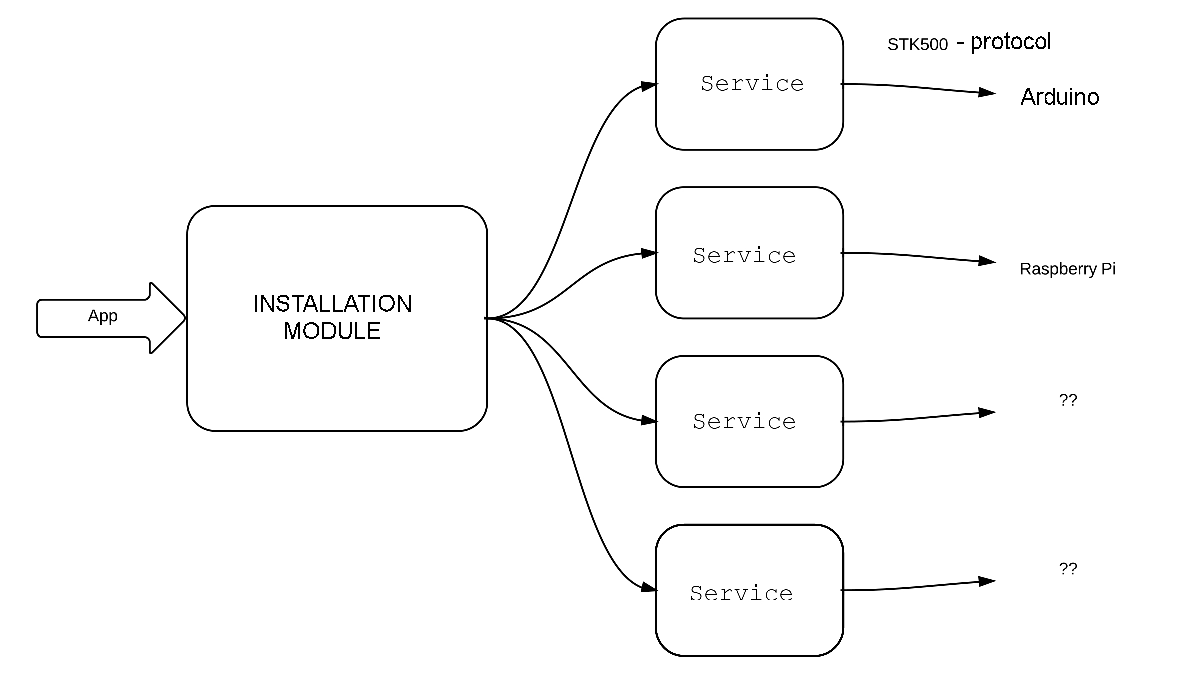
\includegraphics[scale=0.7]{figures/OTAArchitecture.pdf}
	\caption[Over The Air Architecture]{The installation module is a class that manages all the services that the application will support. Each service has a protocol for installing over-the-air to a desired microcontroller.}
	\label{fig:otaarchitecture}
	\end{figure}

	The overall system architecture as shown in Figure~\ref{fig:systemarchitecture} illustrates the core components of the system and the relationship between these components. The \textit{Market Application} is the center of the application and is where most the GUI and functionality to the user is taking place. \textit{Device List} is the list of devices that the user can choose from and connect to. It is also here the \textit{Add Device} functionality is, where the user can connect to a device on an alternative way (QR Code or MAC-address).\\

	\begin{figure}[H]
	\centering
	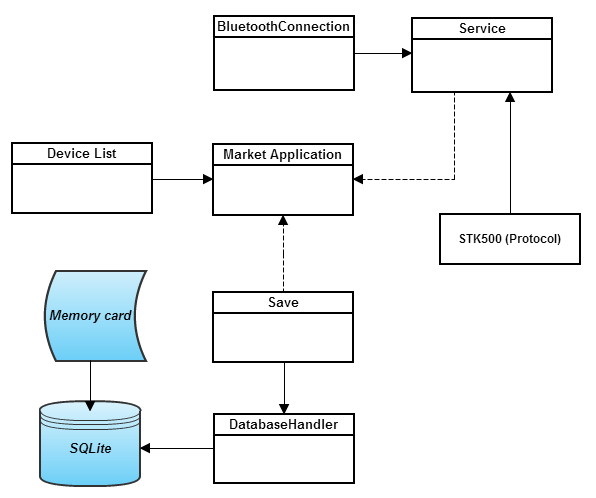
\includegraphics[scale=0.8]{images/System_architecture.png}
	\caption[System Architecture]{This shows the overall system architecture with the most important components.}
	\label{fig:systemarchitecture}
	\end{figure}

	The \textit{Market Application} is the center of the application and is where most the GUI and functionality to the user is taking place. \textit{Device List} is the list of devices that the user can choose from and connect to. It is also here the \textit{Add Device} functionality is, where the user can connect to a device on an alternative way (QR or MAC-address). This is illustrated in Figure~\ref{fig:adddevicescreenuml} \\

	\begin{figure}[H]
	\centering
	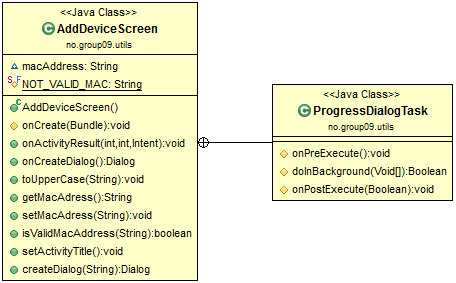
\includegraphics[scale=0.85]{images/UML/adddevicescreen.png}
	\caption[UML - AddDeviceScreen]{This is a UML diagram of Add Device Screen. When QR-reader or input-serial is chosen, a new asynchronous task is started that handles the bluetooth connection process.}
	\label{fig:adddevicescreenuml}
	\end{figure}

	The \textit{Service} holds and manages the bluetooth connection (\textit{BluetoothConnection}) and is taking care of the protocol for installing apps on the microcontroller. \\

	The \textit{Memory card} is the memory card on the mobile phone where the database is stored (locally). SQLite was used for database engine because it is common and easy to implement in Android.\\

	\textit{DatabaseHandler} is a class for taking care of the SQL transactions and is the access point for communication with the database. A helper class called \textit{Save} is used for easy access to the \textit{DatabaseHandler}.
	When the application communicates with the Save module, the database communicates with the DatabaseHandler.
	\textit{Save} was created because it can be initialized and created everywhere in the application (in optional java classes) and makes sure its only one instance of the \textit{DatabaseHandler}.

	\subsection{Browse Shop}
	This is the shop where the user can see the $\mu$C apps, choose categories and swipe though different fragments. In  Figure~\ref{fig:categoriesuml} we see the \textit{MainActivity} that is the activity for the category selection of the shop. 
	When a category is selected, a new activity \textit{MainFragmentActivity} (see Figure~\ref{fig:maingui}) is started with the intent information about which category that was selected.

	\begin{figure}[H]
	\centering
	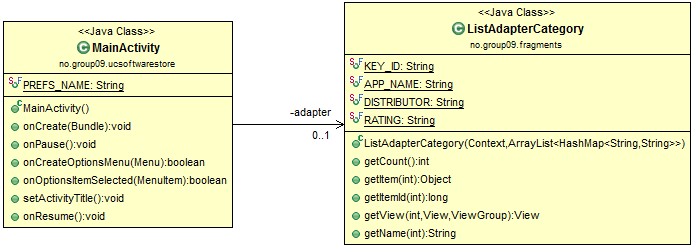
\includegraphics[scale=0.85]{images/UML/categories.png}
	\caption[UML - Categories]{The MainActivity is an activity with a ListView that uses ListAdapterCategory as an adapter. When a category is selected, the ``MainFragmentActivity'' is started with intent information about which category that was selected.}
	\label{fig:categoriesuml}
	\end{figure}

	In Figure~\ref{fig:maingui} the \textit{MainFragmentActivity} is started when a category is selected. This activity creates an FragmentPagerAdapter that manages the fragments. One fragment is one of the views that can be swiped thorugh. \textit{All} and \textit{TopHits} are these fragments. Each fragment consist of a list, and have an Adapter for this list (ListAdapter).

	\begin{figure}[H]
	\hspace*{-1.0in}
	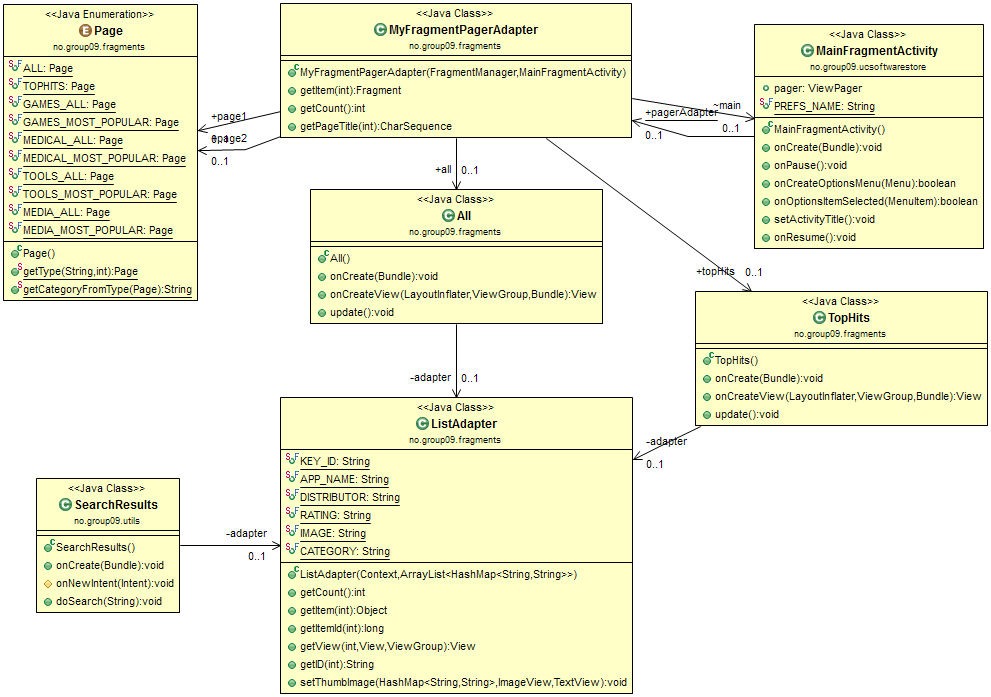
\includegraphics[scale=0.55]{images/UML/main.png}
	\caption[UML - Main GUI]{Here we see a FragmentPagerAdapter that manages all the fragments. Each fragment uses an ListAdapter that structures the list items.}
	\label{fig:maingui}
	\end{figure}

	The \textit{Page} enum is used to tell \textit{MyFragmentPagerAdapter} which category that should be shown in \textit{All} and \textit{TopHits} fragments. This enum is sent as a intent to the MainFragmentActivity when started. When a category is chosen, the content in \textit{All} and \textit{TopHits} are filtered by only showing applications that belongs to the selected category.\\

	\textit{SearchResults} is a class that contains a list of search results ($\mu$C applications) from the search. This class is an activity that have a list like the other fragments, and therefore uses the same list adapter as \textit{All} and \textit{TopHits}. 

	\subsection{STK500v1}
	In Figure~\ref{fig:stk500v1uml} the general design of the protocol component is shown. The STK500v1 class
    handles most of the logic and actual programming; this is the class called upon by the application when
    an app is to be uploaded. The Constants class holds important commands and responses used when communicating
    with the Arduino.
    The Hex class deals with interpreting and verifying the app to be programmed. It provides the raw bytes
    requested by the protocol class.\\
    
    The rest are for abstracting and dealing with reading from the Bluetooth connection; the current
    implementation allows for avoiding blocking by only reading buffered bytes. The Reader behaves differently while
    %TODO: reference state pattern
    reading or during timeouts, based on a state pattern implementation. As shown, the different states are both
    states and readers.\\

	\begin{figure}[H]
	\hspace*{-1.0in}
	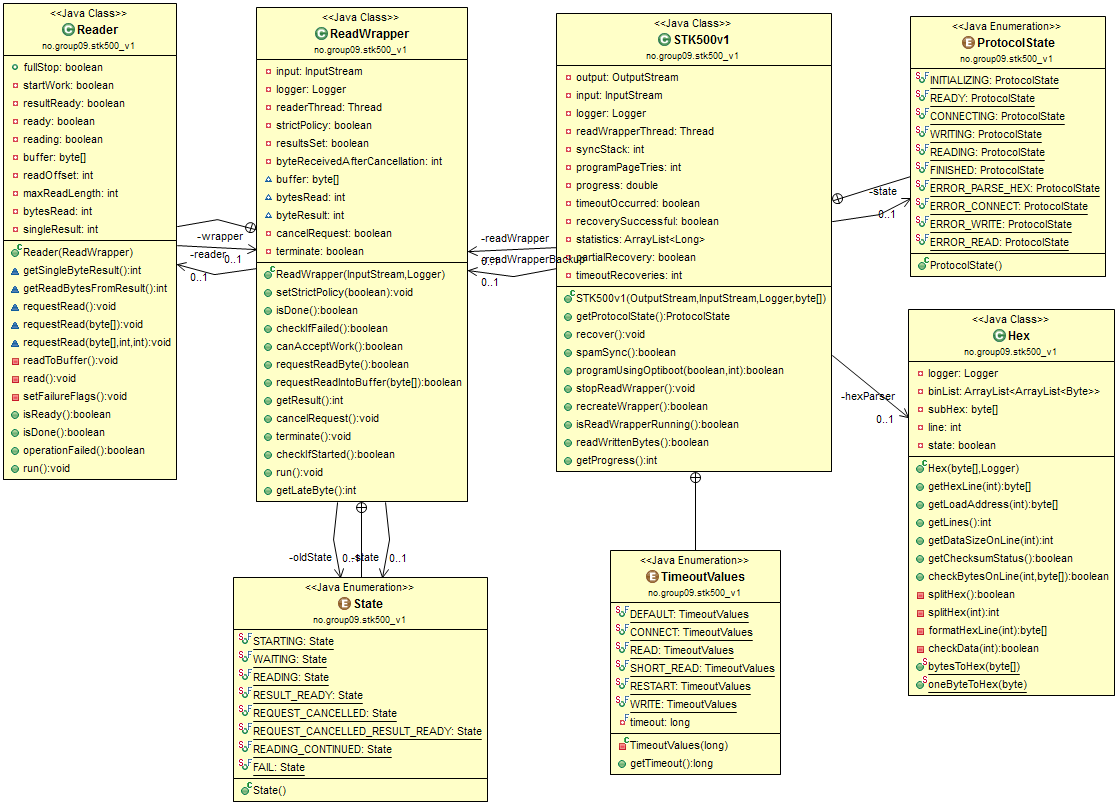
\includegraphics[scale=0.58]{images/UML/stk500v1.png}
	\caption[UML - Protocol]{The most important classes used for programming}
	\label{fig:stk500v1uml}
	\end{figure}

	In Figure~\ref{fig:stk500_sequence_diagram} a simplified view of the programming process is shown. ArduinoStore is here a representation of any application requesting an app to be uploaded to the Arduino,
	and the Arduino represents a microcontroller to be programmed.\\
	
	Note that the IReader has already been instantiated before the starting call, and that stopping doesn't
	destroy the object.\\
	
	Most of the simplification occurs within the programming loop, as several different types of commands
	are sent to the device, depending on the responses received; for details on this communication, see the AVR061 documentation~\cite{AVR061}. Communication details with the Hex class and IReader-related classes have also been reduced slightly in the diagram.\\
	
	\begin{figure}[H]
	\hspace*{-1.0in}
	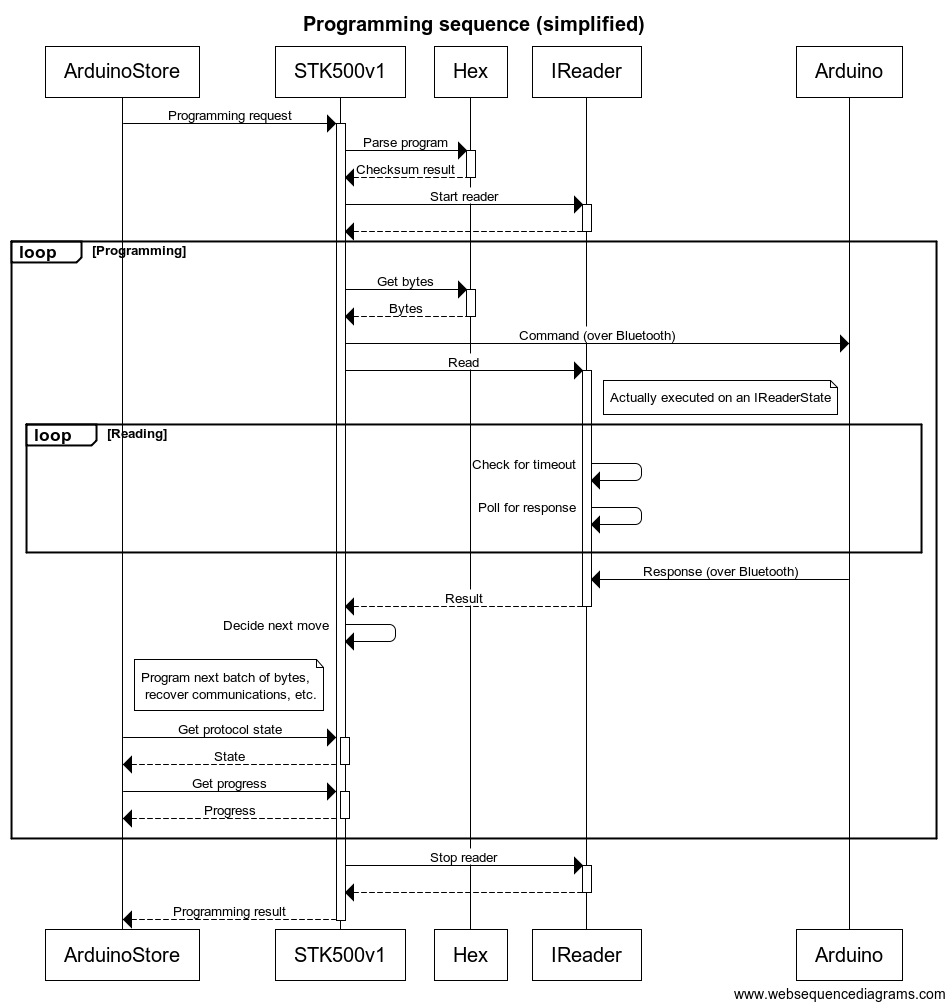
\includegraphics[scale=0.6]{images/Sequence_diagram.png}
	\caption[Sequence diagram for programming]{Sequence diagram of the programming process. The three classes in the middle are in the protocol library, ArduinoStore represents an outside caller, and the Arduino is a programmable microcontroller.}
	\label{fig:stk500_sequence_diagram}
	\end{figure}


\section{Design of Android application}
One of the purposes of the Android application was to ease the process of installing PUIs on an Arduino for non-technical users. As described in section \ref{non-functional}, one of the requirements for the project was that people of all ages are supposed to understand how to use the application. This requirement put pressure on the design, as one have to make sure everyone are able to understand the different functions of the application. \\
\newline
Before the programming of the Android application was started, a complete design guide were created. In this section the complete design of the application is presented. This guide was made for primarily two reasons:
\begin{itemize}
	\item{Presentation for the customer:} With a complete design guide it was possible to present the user interface of the application to the customer before it was programmed. This allowed for input from the customer at an early stage, when it was easier to change the design.
	\item{Avoid confusion:} A design guide reduces the amount of confusion and discussion regarding the appearance of the user interface. When the looks of the user interface was settled before the programming had started, there was less need to discuss this along the way.
\end{itemize}

\subsection{Design guide}
Following is the complete design guide of the Android application. Minor changes were made to some of the screens. In these cases it is commented below the picture. The design of the preferences screen is not shown, as it was unnecessary to design this screen since it is a standard for Android applications.

\paragraph{Screen 1a - Device list}
Screen that shows the list of available Arduino devices. In the final design the list of devices fills the whole screen, and the buttons and description text have switched places. When a device is clicked, a progress bar appears and stays on the screen until a valid Bluetooth connection with the chosen device is made.

\begin{figure}[H]
	\centering
		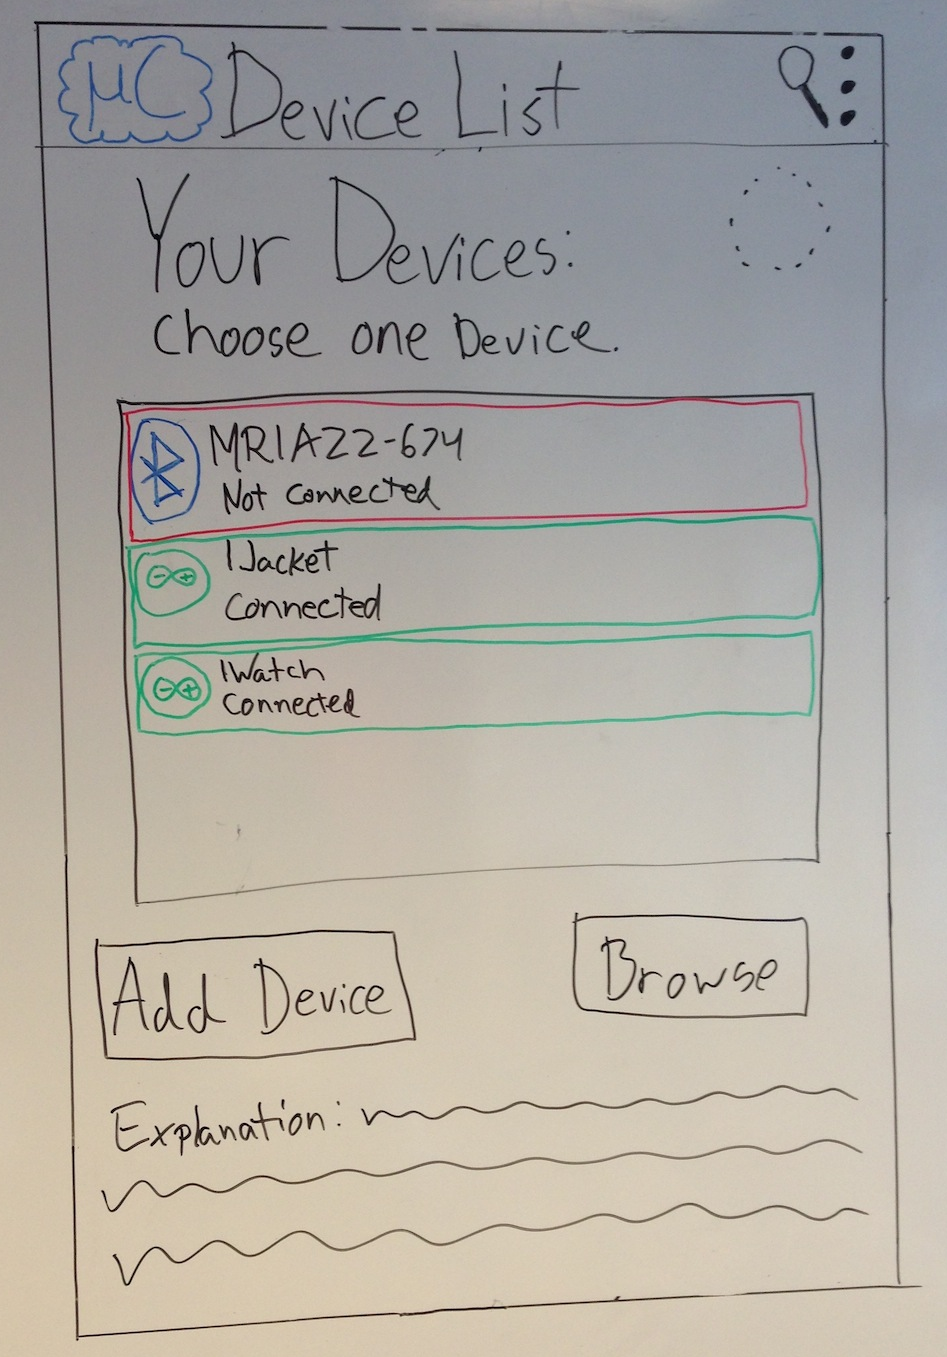
\includegraphics[scale=0.2]{images/Design_guide/Screen1a.png}
	\caption[Screen 1a - Device list]{The design for the device list of the discovered bluetooth devices}
	\label{fig:screen1a}
\end{figure}


\paragraph{Screen 1b - Add device manually}
Screen that appears after pressing the ``Add device'' button in Screen 1a. It was chosen to remove the ``Bluetooth settings'' button, as it proved unnecessary. In the final design, this screen contains only the ``QR code'' button and ``Input serial'' button, with a short description of the functionality of the button between them.

\begin{figure}[H]
	\centering
		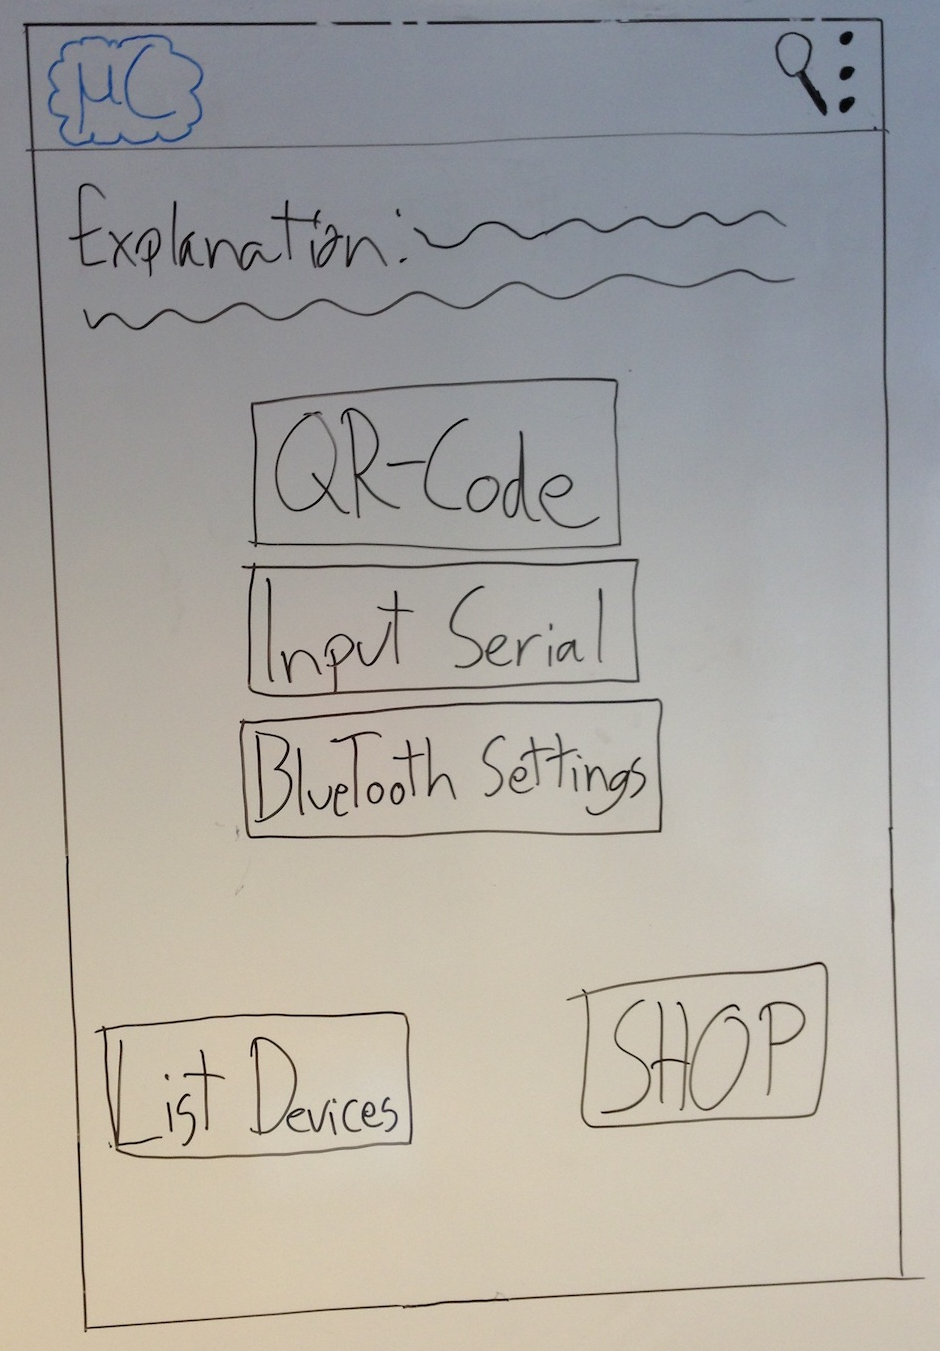
\includegraphics[scale=0.2]{images/Design_guide/Screen1b.png}
	\caption[Screen 1b - Add device manually]{The design for how to add devices alternatively}
	\label{fig:screen1b}
\end{figure}


\paragraph{Screen 1b-i - Input serial}
Screen that appears when the ``Input serial'' button is clicked.

\begin{figure}[H]
\centering
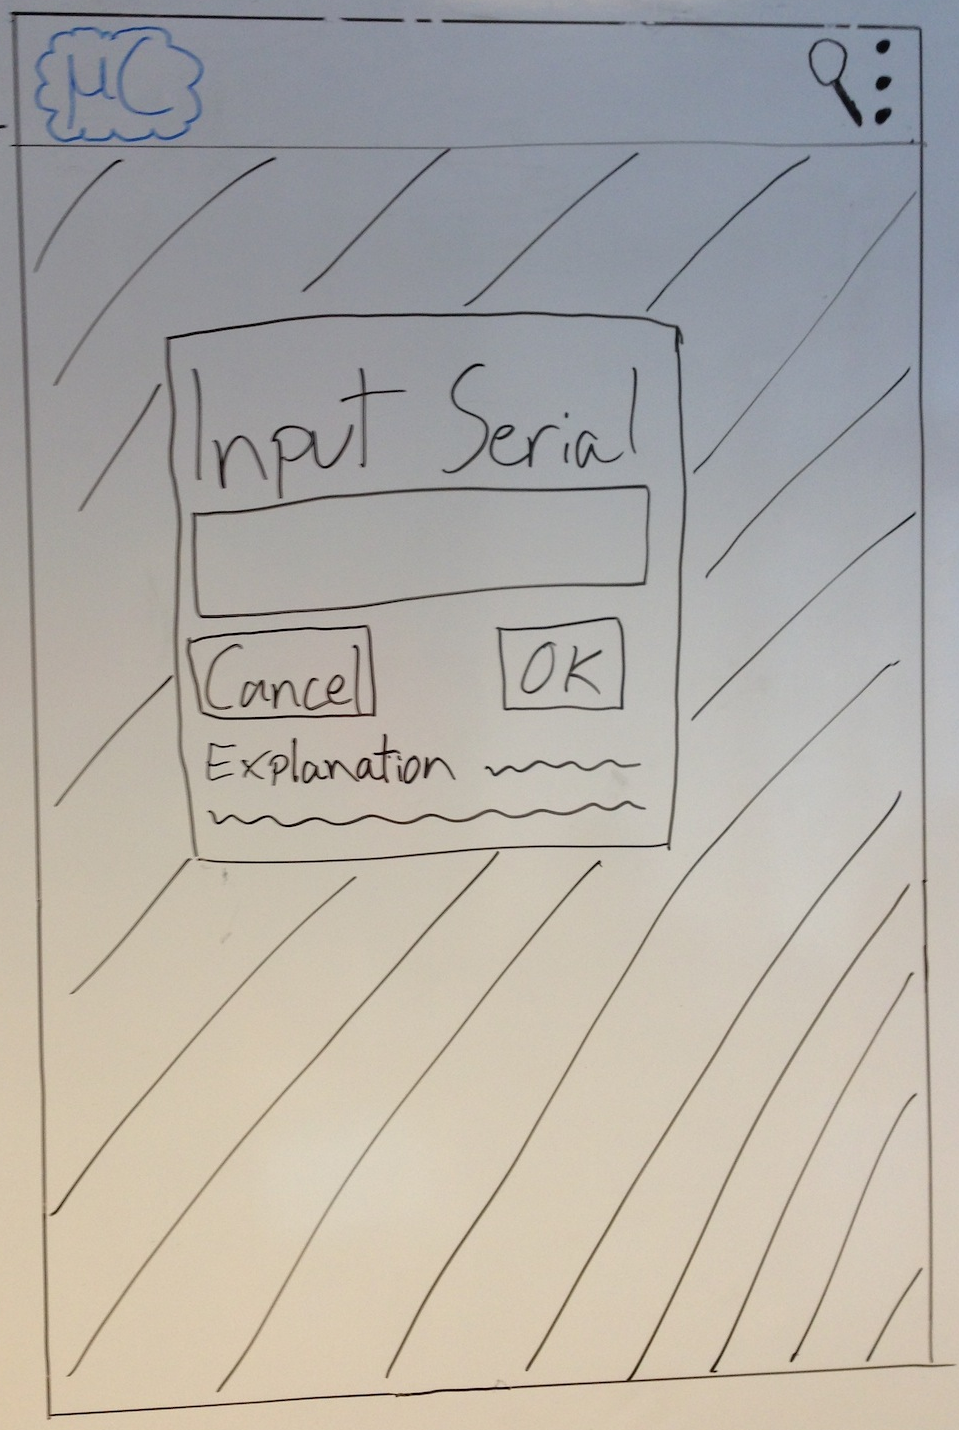
\includegraphics[scale=0.2]{images/Design_guide/Screen1b-i.png}
\caption[Screen 1b-i - Input serial]{The design for input serial popup box.}
\label{fig:screen1bi}
\end{figure}


\paragraph{Screen 2a - Browse shop}
Screen for browsing all the applications for Arduino in the shop. More categories have been added. The user can here swipe left/right to sort the available applications in different ways. See next paragraph.

\begin{figure}[H]
\centering
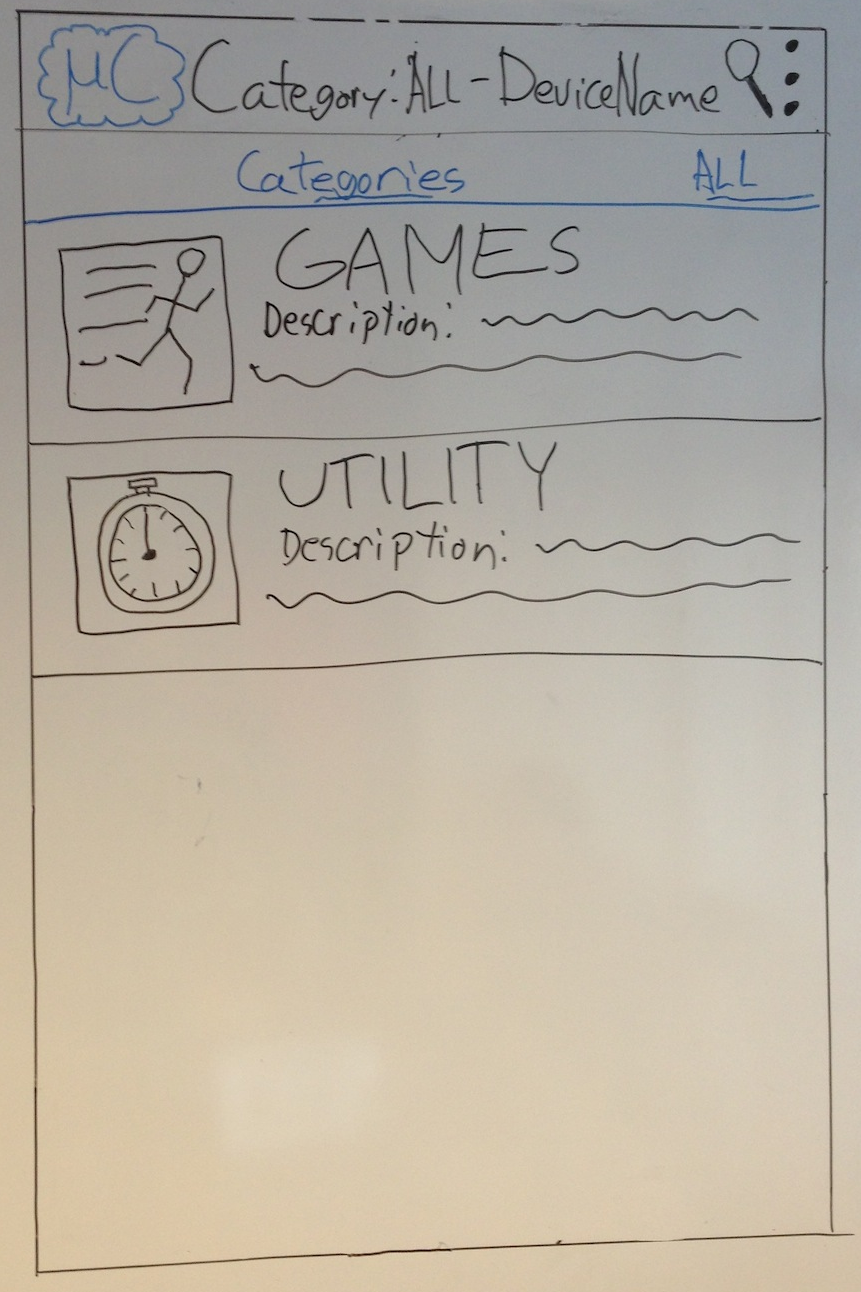
\includegraphics[scale=0.2]{images/Design_guide/Screen2a.png}
\caption[Screen 2a - Browse shop]{Design for category selection in the shop.}
\label{fig:screen2a}
\end{figure}


\paragraph{Screen 2b - Browse shop by category}
Screen that shows a list of all applications in chosen category. Category ``All'' is chosen.

\begin{figure}[H]
\centering
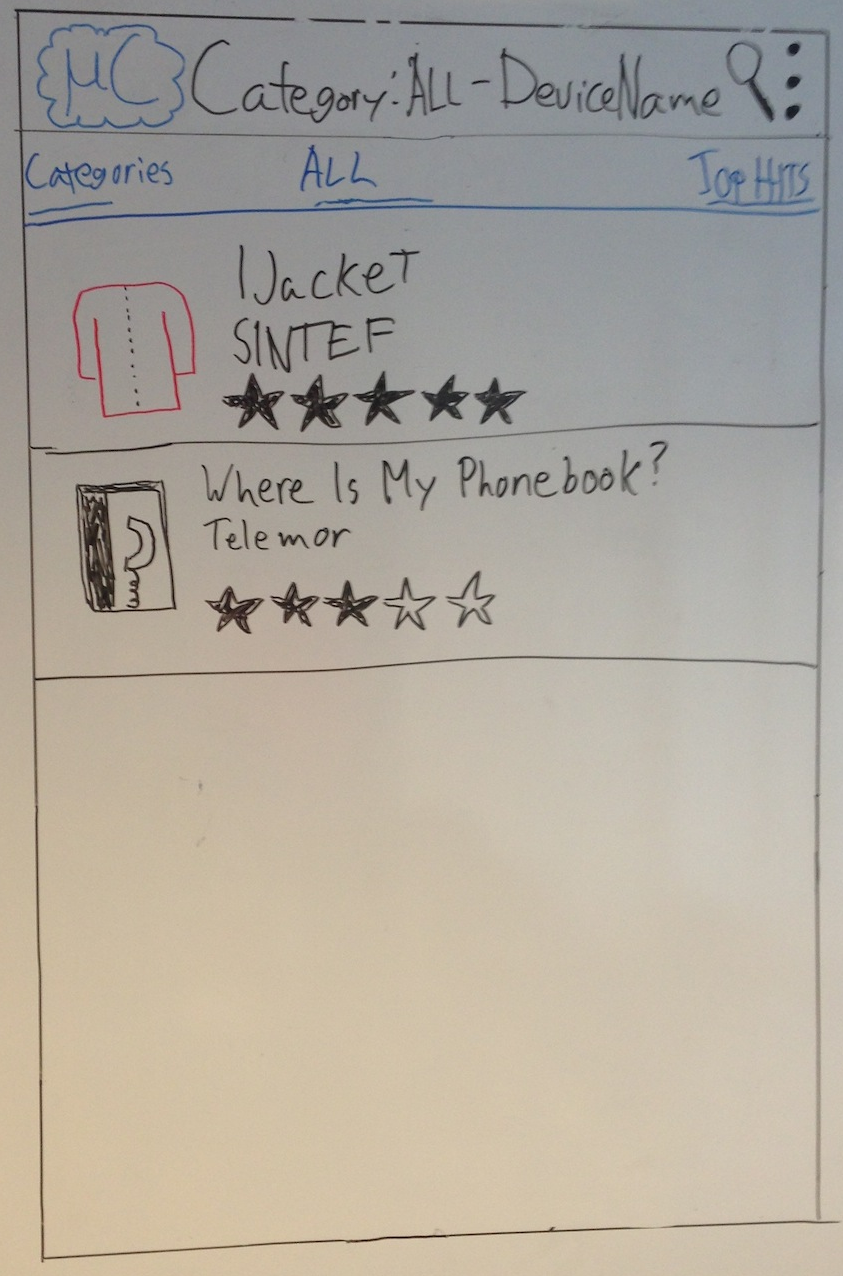
\includegraphics[scale=0.2]{images/Design_guide/Screen2b.png}
\caption[Screen 2b - Browse shop by category]{Design for the list of application that belongs to the selected category.}
\label{fig:screen2b}
\end{figure}


\paragraph{Screen 3a - Application view}
Screen with overview of an chosen application. Small changes were needed, as the comments field and reviews were given a lower priority at mid-term.

\begin{figure}[H]
\centering
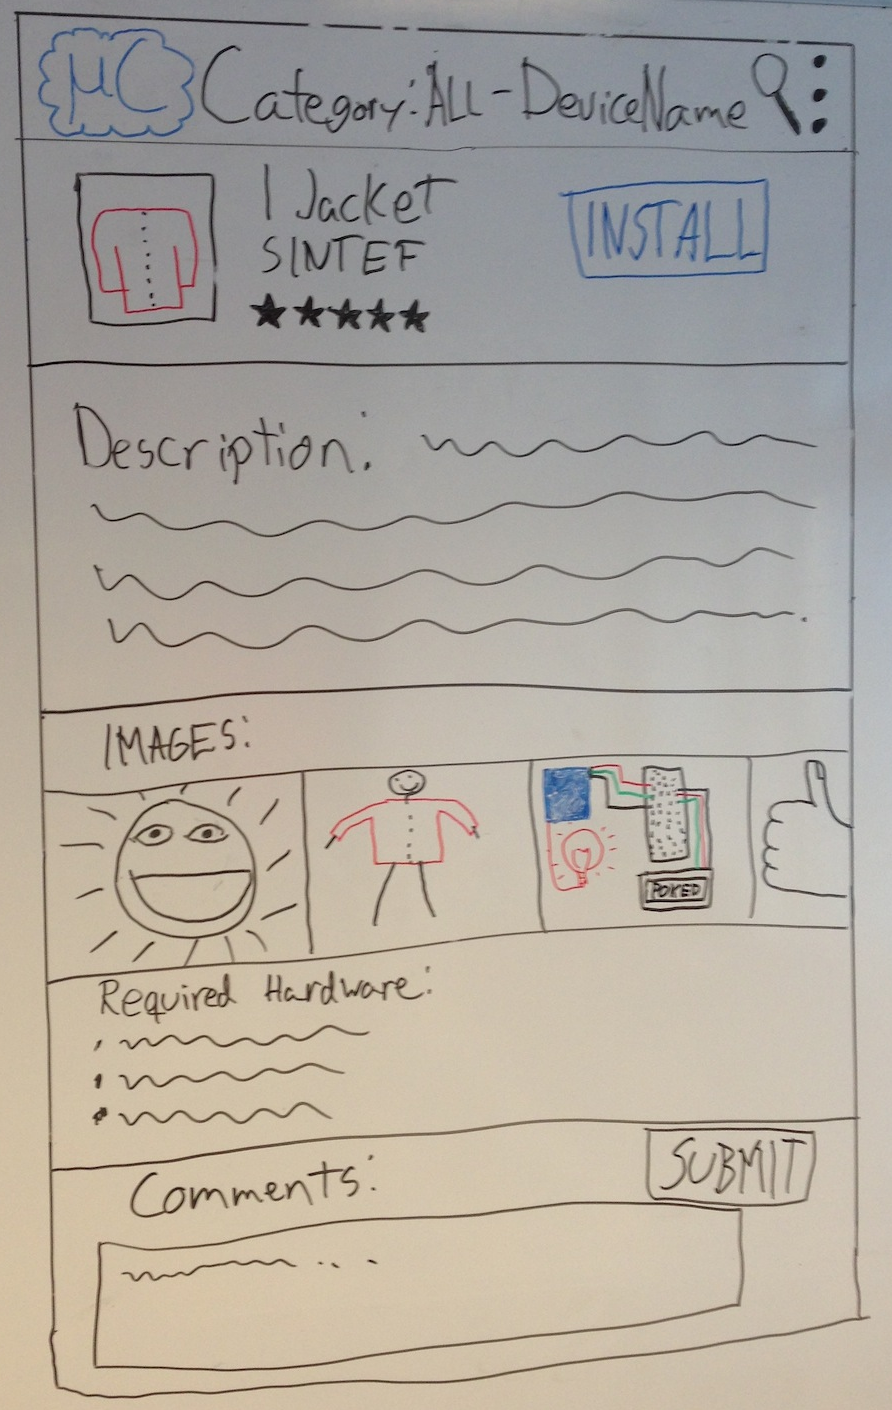
\includegraphics[scale=0.2]{images/Design_guide/Screen3a.png}
\caption[Screen 3a - Application view]{The design for application view. This is the screen you see when you look at the details about an application}
\label{fig:screen3a}
\end{figure}


\paragraph{Screen 3a-i - Installation confirmation}
Screen that appears when the ``Install'' button in Screen 3a is pressed. Shows the name of the chosen device.

\begin{figure}[H]
\centering
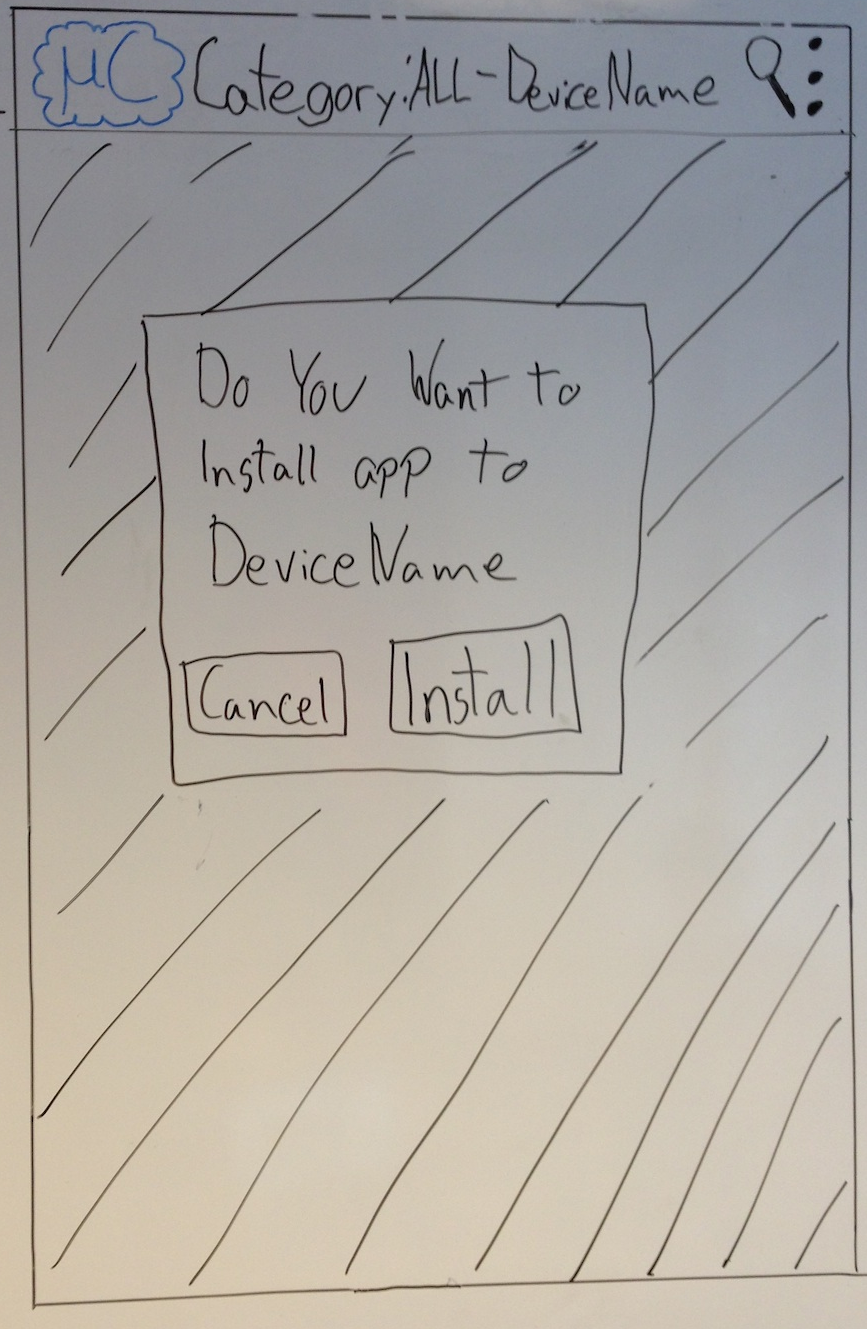
\includegraphics[scale=0.2]{images/Design_guide/Screen3a-i.png}
\caption[Screen 3a-i - Installation confirmation]{When the user click ``install'' , this box will show up to warn and confirm the users choice}
\label{fig:screen3ai}
\end{figure}


\paragraph{Screen 3a-ii - Progress of installation}
Screen that shows the progress of the installation. The progress bar cannot be dismissed, so the Android application is locked until the installation is complete or has failed.
The user is warned not to move the Android device out of range of the Arduino.

\begin{figure}[H]
\centering
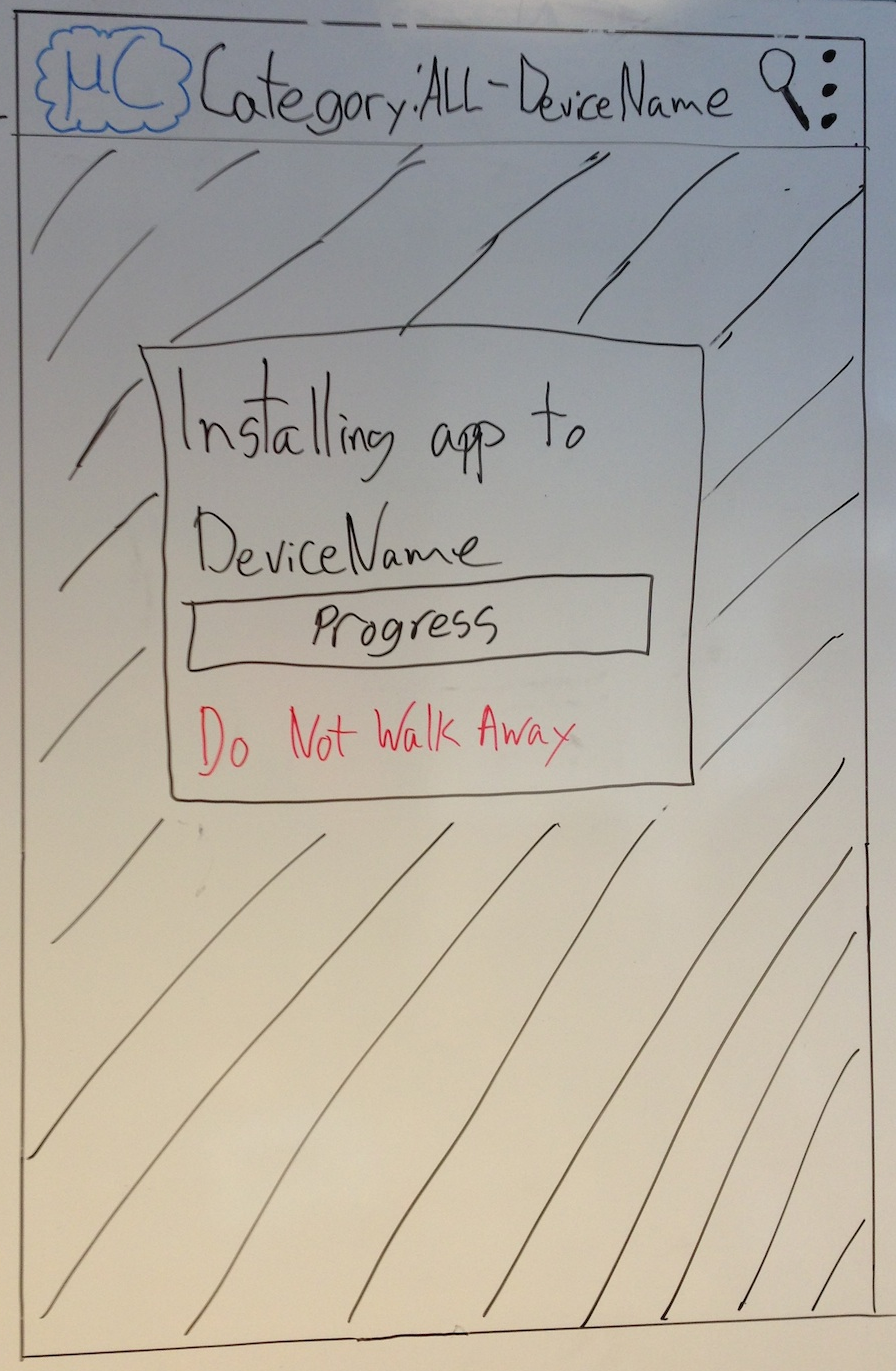
\includegraphics[scale=0.2]{images/Design_guide/Screen3a-ii.png}
\caption[Screen 3a-ii - Progress of installation]{The progressbar that will shop up during the installation over-the-air.}
\label{fig:screen3aii}
\end{figure}


\paragraph{Screen Xa - Action overflow}
Screen that appears when the ``Action overflow'' button is clicked. This menu is available from all the screen in the application with the exception of the preferences screen.

\begin{figure}[H]
\centering
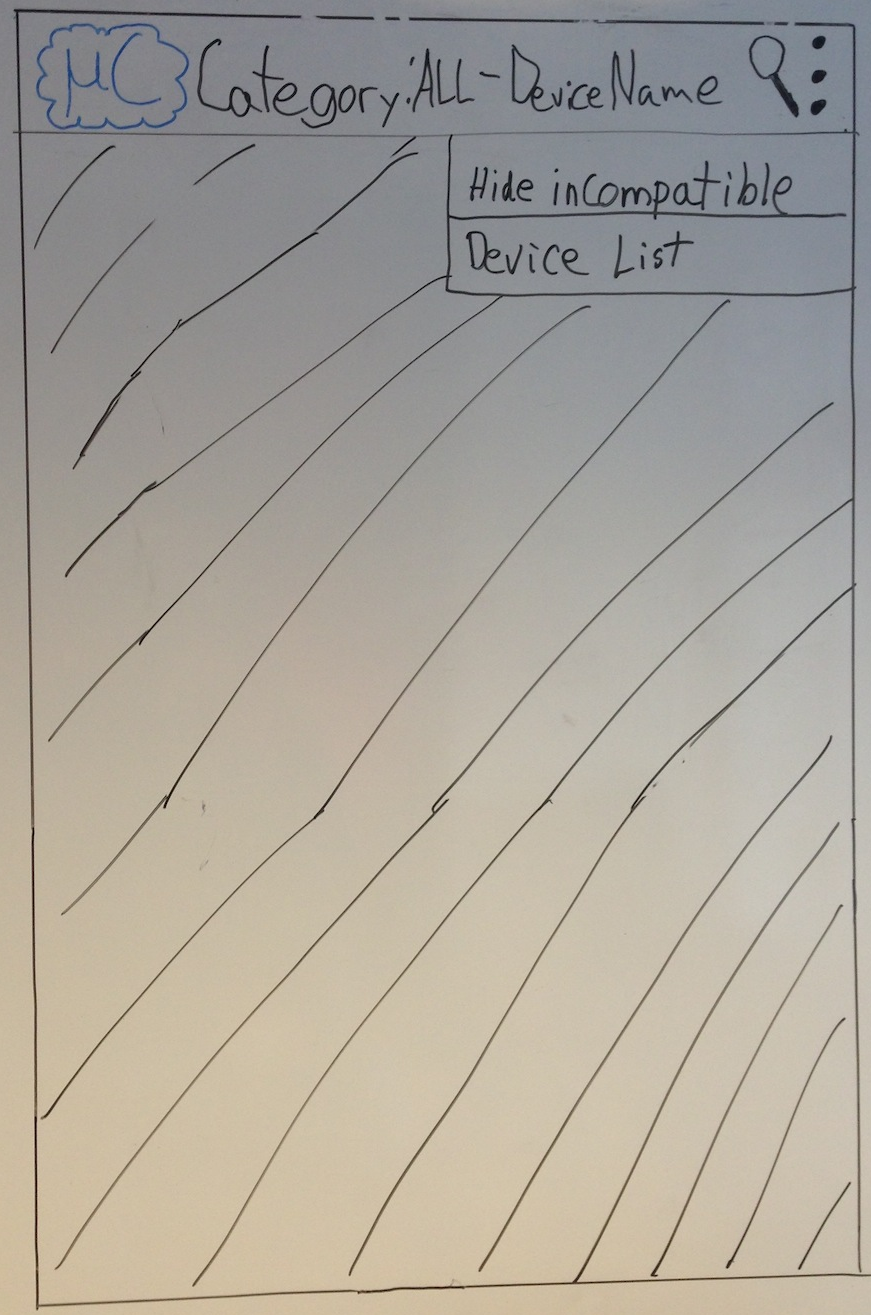
\includegraphics[scale=0.2]{images/Design_guide/ScreenXa.png}
\caption[Screen Xa - Action overflow]{The menu bar that contains settings and properties.}
\label{fig:screenXa}
\end{figure}

	\subsection{Design decisions}
	This section explains the reasoning behind the different aspects of the design.

	\textbf{Device list}\\
	It should be simple and fit as many devices as possible, even on the smaller cell phones. As shown in Figure~\ref{fig:screen1a} it was decided to use discovered Bluetooth devices as a primary method of connection to an Arduino. That is why the user will meet this screen first. The less frequently used methods for connecting to an Arduino, like QR codes and serial input, were therefore put separately in another screen, as shown in Figure~\ref{fig:screen1b}. \\

	Because of license compatibility issues, it was necessary to use external QR Code readers. To give the user more flexibility, it is therefore possible for the user to select the optimal QR-reader from his application list.\\

	When serial input is clicked, it was decided to open a dialog box for the input string as shown in Figure~\ref{fig:screen1bi}. This is because it clearly gives the user feedback on what is happening and it does not add unnecessary clutter to the GUI.\\

	\textbf{Browse shop}\\
	The category selection as shown in Figure~\ref{fig:screen2a} was done because it groups the applications, and makes it easier for the user to browse for the more specific applications. The swiping was implemented because it easily and quickly selects what to show. This is a fast way to change what to sort the applications by, and is user friendly on a touch screen. ``Top hits'' and ``All'' were chosen because the database is currently small, and it is not necessary with a large amount of ``sort by'' tabs. Other tabs could be easily implemented if need be.\\

	\textbf{Application view}\\
	The application view, as shown in Figure~\ref{fig:screen3a}, should show all the detail and information about an application that is useful and interesting to the user. Rating, description, developer, application name and images were selected for trying to keep a ``standard''. Meaning that both Google Market and AppStore uses these elements and are expected to be familiar for many users.\\

	When the install button is clicked a confirmation box will pop up as shown in Figure~\ref{fig:screen3ai}. This is because the user might have clicked the button on accident or is not informed about what device he/she is connected to. The device name will therefore be shown in this dialog box.\\

	A progress bar will pop up when the user have confirmed the installation. This is because the application should give an indicator on when the application is complete and when its safe to close the application. \\

	\textbf{Action overflow menu}
	When the user clicks on the action overflow menu, he will expect some sort of settings. That is why this menu contains settings. If the user will hide or show incompatible application to his Arduino, this menu will toggle the preference as shown in Figure~\ref{fig:screenXa}.\\

	\textbf{Changes to the design}
	The action overflow menu have two other options: ``Device List'' and ``Populate Database''. This is because this application is only a prototype and it was necessary to hard code Arduino applications into the Android application. The populate database function will therefore feed the local database with some sample applications.\\

	The device list function is there because it should be possible to change device at all times, not only on startup.\\

	Another change is the ``Welcome Screen''. This is the first screen that will be met when the application is started. This makes it easier to navigate between ``Devices'' and ``Browse Shop''. This screen also provides an option (checkbox) that allows the user to chose wheter or not they will automatically reconnect on startup. Figure~\ref{fig:welcomescreen} shows a simple connection between the reconnect option and the welcome screen.

	\begin{figure}[H]
	\centering
	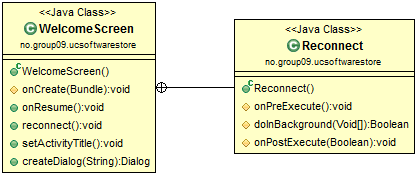
\includegraphics[scale=0.85]{images/UML/welcomescreen.png}
	\caption[UML - Welcome Screen]{The Welcome Screen will reconnect to last connected device if the user have this option enabled. When the user clicks on ``Devices'' or ``Browse Shop'' a new activity is started.}
	\label{fig:welcomescreen}
	\end{figure}

\section{Database implementation}

	SQLite was used as database language because it is integrated with Android and have much functionality that makes it easy to use in an Android application. Because of changes to priorities the group and the customer got in an agreement to drop the sync adapter, and only use a local database.

	\subsection{Database model}

		In figure~\ref{fig:erdiagram} the database is shown as an ER Diagram. The pictures table was not used because of changes to the teams priorities. Things that had been done before was not important for the customer.

		\begin{figure}[H]
		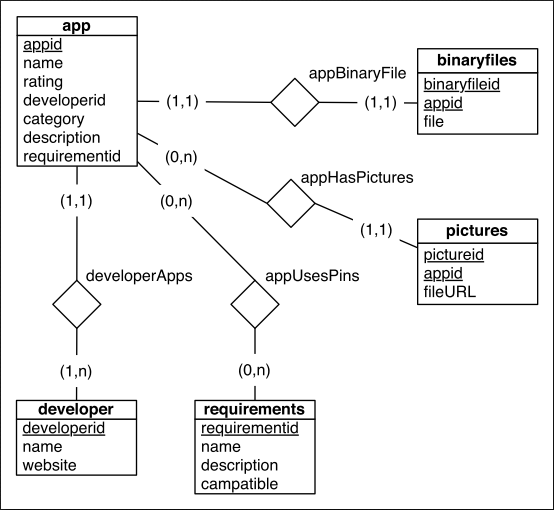
\includegraphics[scale=1]{images/ER_Diagram.png}
		\caption[ER Diagram]{The ER Diagram describing the setup of the app database.}
		\label{fig:erdiagram}
		\end{figure}

	\subsection{Database details}

		Description and detail about the database tables.

		\subsubsection{Table: app}

			This table contains information about the application.\\

			{\bf \underline{appid}(integer):} auto-increment primary key for applications  \\
			\textbf{name(varchar 160):} name of the application \\
			\textbf{rating(int 10):} rating of the application \\
			\textbf{developerid(int 10):} foreign key to the developer of this application \\
			\textbf{category(varchar 200):} which category this application belongs to \\
			\textbf{description(varchar 200):} description of the application \\
			\textbf{requirementid(int 10):} foreign key to the requirements of this application \\

		\subsubsection{Table: binaryfiles}

			This table contains information about the hex-file (compiled Arduino code). \\
			
			{\bf \underline{binaryfileid}(integer):} auto-increment primary key for binary files \\
			\textbf{appid(int 10):} foreign key to the application that owns this binary file \\
			\textbf{file(BLOB 1000000):} The binary file in a BLOB \\

			A BLOB is not a datatype and stores data exactly as it was input. This database stores it as a binary array.

		\subsubsection{Table: developer}

			This table contains information about the developer.\\
			
			{\bf \underline{developerid}(integer):} auto-increment primary key for developers \\
			\textbf{name(varchar 160):} name of the developer \\
			\textbf{website(varchar 200):} website of the developer \\

		\subsubsection{Table: requirements}

			This table contains the requirements for the application.\\
			
			{\bf \underline{requirementid}(integer):} auto-increment primary key for the requirement \\
			\textbf{name(varchar 160):} name of the requirement \\
			\textbf{description(varchar 200):} description of the requirement \\
			\textbf{compatible(int 10):} integer that is converted to boolean when retrieved from database. \\

			Compatible is an integer of 1 or 0. This indicates if the application referred to is compatible with pagers or not.

		\subsubsection{Table: appusespins}

			This table contains the information about which pins on the Arduino that the application is using.\\
			
			\textbf{appid(int 10):} foreign key to the application that uses this rule \\
			\textbf{requirementid(int 10):} foreign key to the associated requirement \\


\chapter{Testing}
	This chapter contains a description of the testing performed during the project. Tests were performed in order to ensure product quality and that the product met the requirements set.
	
	\section{Testing strategy}
		The ways in which testing was performed is detailed in this section. Testing was performed by unit testing first, then integration testing. Usability testing was performed after the main shop part of the project was completed. User acceptance testing was then performed by the customer after significant parts were complete. \cite{testing-overview}

		\subsection{Unit testing}
			For testing of the Android application, Robotium was used. Robotium is a powerful test framework that can be used for function, system and acceptance testing. The tests created in Robotium aims at writing small portions of code and checking the results against expected predefined values. Robotium was used for unit testing on the Android application. During the development of the application, different units were tested with Robotium after they were finished. An example of a Robotium test is shown below. In this test it is asserted that the Bluetooth connection with a Arduino device is as expected. \cite{unit-testing1} \cite{unit-testing2} \cite{unit-testing3} \\

			\begin{lstlisting}
solo.clickOnActionBarItem(R.id.settings);

ConnectionState expectedState = BluetoothConnection
	.ConnectionState.STATE_CONNECTED;
	
ConnectionState actualState = BtArduinoService.getBtService()
	.getBluetoothConnection().getConnectionState();

assertEquals(expectedState, actualState);
			\end{lstlisting}

		\subsection{Integration testing}
		Integration testing is based on combining different units and testing the interface and communication between them. This type of testing comes after the unit testing phase and before the validation testing. The units that can be used in these tests must therefore have passed the unit tests. This made integration testing focus purely on the integration of units rather than having tests to ensure the units work correctly as well. Because the system is composed of more than one component (STK500 protocol and the Android application), they were tested in pairs and not all at once. Integration testing identifies problems that occur when we combine the different units of the product, and was performed when units of the product was put together.\\ \cite{integration-testing1} \cite{integration-testing2}
		\newline
		Just as in unit testing, Robotium was used for integration testing as well. This is well supported as you can code the test to press different buttons or text and are therefore capable of navigating through the entire application, and/or units.\\

		\subsection{Usability test}
		As the intent of the product was to ease the use of and set up physical user interfaces, usability tests were crucial in the testing aspects. The decision were made to perform a hallway test following tasks given to the test subjects. To ensure that the test subjects had a proper understanding of the product, the think aloud protocol was used, meaning the subject talked about their actions during the test. \\
		\newline
		All test subjects filled out a System Usability Scale (SUS) form in order to create a score, 0-100, which gave us a comparable score with other systems. Concerning the amount of subjects tested, five users has been recognized as the proper amount. According to \cite{Nielsen}, 85\% of the problems with a system will be found by these five users, thus testing more would increase the time spent watching the same problems resurface.

		\subsubsection{Tasks}
			These were the tasks given to each tester. The tasks were created with the user cases previously mentioned as a basis. Each task is meant to be a vague description of what they are supposed to do in order for them having to think mostly for themselves and not given any answer as to what they are supposed to do.

			The preface of these tasks was that they had bought a jacket with an Arduino device fitted in it. This jacket was called an iJacket and they had just downloaded the $\mu$CSS in order for them to check what other applications they could have on this jacket.

			\vspace{6 mm}
			\begin{enumerate}
			 \item Select your jacket
			 \item Look for applications
			 \item Install the application
			\end{enumerate}
			\vspace{6 mm}

			After the tests the test subjects were asked if there were any details or points during the test where they either were confused or found it difficult to do something. These points would be added or confirmed on a form where the observer would have noted any other details which may have risen during the test.

		\subsection{User acceptance testing}
		User acceptance testing was performed with the customer in order to ensure that requirements were met and to check whether or not the customer was satisfied. This test was done in much the same way as the usability test, though with a scope bigger than just the usability aspect. A phone with the application was given to the customer in order for him to get first degree experience with the application. The tester was then asked to perform the same cases as in the usability tests, while thinking aloud in order to properly record his reactions to the application. These reactions were then written down on paper. After the cases were done with, the customer was given the opportunity to just play around with the product. Lastly, the customer was asked to what degree he felt the product fulfilled the requirements set for the product.\\
		\newline
		There were also expert reviews made during a presentation at the offices of SINTEF. The think aloud protocol was also used here. These testers had much experience within development, but not much knowledge about the task. They were therefore given a brief presentation beforehand about the project and given a short presentation of the application itself.\\


	\section{System Testing}
	\label{systemtesting}
	In this section the system tests will be presented. Each test was written to test a specific part of the product, and applies to both the Android application, STK500 protocol and software installed on the Arduino device. Each test was executed separately, and the results will be presented in section \ref{testresults}.

	\begin{table}[H]
	\caption{Connect with device using device list}
	\begin{tabularx}\linewidth{|m{0.15 \textwidth}|X|}
		\hline
			{Test ID} & {ST01}\\
		\hline
			Test name & Device list connect\\
		\hline
			Test description & Connect with an Arduino device from the Device list screen \\
		\hline
			Precondition & Arduino device is switched on with Bluetooth \\
		\hline
			Test steps & \begin{itemize}
				\item{Start program}
				\item{Press Device list from Action overflow or from the Welcome screen}
				\item{Press desired Arduino device}
				\end{itemize} \\
		\hline
			Success condition & Android and Arduino device is connected via Bluetooth \\
		\hline
	\end{tabularx}
	\end{table}

	\begin{table}[H]
	\caption{Connect with device using QR code}
	\begin{tabularx}\linewidth{|m{0.15 \textwidth}|X|}
		\hline
			{Test ID} & {ST02}\\
		\hline
			Test name & QR code connect\\
		\hline
			Test description & Connect with an Arduino device using QR code reader \\
		\hline
			Precondition & Arduino device is switched on with Bluetooth \\
		\hline
			Test steps & \begin{itemize}
				\item{Start program}
				\item{Press Device list from Action overflow}
				\item{Press Add device}
				\item{Press Connect with QR code}
				\item{Choose QR code reader}
				\item{Scan QR code}
				\end{itemize} \\
		\hline
			Success condition & Android and Arduino device is connected via Bluetooth \\
		\hline
	\end{tabularx}
	\end{table}

	\begin{table}[H]
	\caption{Connect with device using serial}
	\begin{tabularx}\linewidth{|m{0.15 \textwidth}|X|}
		\hline
			{Test ID} & {ST03}\\
		\hline
			Test name & Input serial connect \\
		\hline
			Test description & Connect with an Arduino device using serial \\
		\hline
			Precondition & Arduino device is switched on with Bluetooth \\
		\hline
			Test steps & \begin{itemize}
				\item{Start program}
				\item{Press Device list from Action overflow}
				\item{Press Add device}
				\item{Press Connect with QR code}
				\item{Choose QR code reader}
				\item{Scan QR code}
				\end{itemize} \\
		\hline
			Success condition & Android and Arduino device is connected via Bluetooth \\
		\hline
	\end{tabularx}
	\end{table}

	\begin{table}[H]
	\caption{Search for desired app}
	\begin{tabularx}\linewidth{|m{0.15 \textwidth}|X|}
		\hline
			{Test ID} & {ST04}\\
		\hline
			Test name & Search \\
		\hline
			Test description & Search for a specific app \\
		\hline
			Precondition & Database is populated \\
		\hline
			Test steps & \begin{itemize}
				\item{Start program}
				\item{Press search icon}
				\item{Type search string}
				\end{itemize} \\
		\hline
			Success condition & Search result is shown with matching apps \\
		\hline
	\end{tabularx}
	\end{table}

	\begin{table}[H]
	\caption{Connect to last connected device when in range}
	\begin{tabularx}\linewidth{|m{0.15 \textwidth}|X|}
		\hline
			{Test ID} & {ST05}\\
		\hline
			Test name & Last connected\\
		\hline
			Test description & Test that the Android application connects to the last connected Arduino device when it is in range and gives proper feedback to the user. The application should only reconnect when this option is selected. \\
		\hline
			Precondition & Available Arudino device with Bluetooth \\
		\hline
			Test steps & \begin{itemize}
				\item{Check option ''Automatically try to reconnect to last connected device''}
				\item{Connect with an Arduino}
				\item{Exit Android application completely}
				\item{Start Android application}
					\begin{itemize}
						\item{When the Arduino device is in range}
						\item{When the Arduino device is out of range/off}
					\end{itemize}
				\end{itemize} \\
		\hline
			Success condition & When the last connected Arudino device is on and in range, the Android device should connect to it immediately when the Android application is started and give feedback to the user. If the Arduino device is out of range or off, proper feedback should be given \\
		\hline
	\end{tabularx}
	\end{table}

	\begin{table}[H]
	\caption{Browse apps test}
	\begin{tabularx}\linewidth{|m{0.15 \textwidth}|X|}
		\hline
			Test ID & ST06\\
		\hline
			Test name & Browse apps\\
		\hline
			Test description & Browse apps in the Android application in a random fashion \\
		\hline
			Precondition & Database is populated \\
		\hline
			Test steps & \begin{itemize}
				\item{Start program}
				\item{Choose a category}
				\item{Choose an app}
				\item{Go back and choose different app}
				\item{Swipe left/right to browse different sorting}
				\end{itemize} \\
		\hline
			Success condition & User is able to browse apps \\
		\hline
	\end{tabularx}
	\end{table}

	\begin{table}[H]
	\caption{Install application on Arduino device}
	\begin{tabularx}\linewidth{|m{0.15 \textwidth}|X|}
		\hline
			{Test ID} & {ST07}\\
		\hline
			Test name & Install application on Arduino device\\
		\hline
			Test description & Choose a desired application to install on a connected Arduino device \\
		\hline
			Precondition & Android and Arduino device is connected via Bluetooth \\
		\hline
			Test steps & \begin{itemize}
				\item{Start program}
				\item{Select desired app}
				\item{Press Install}
				\item{Press Confirm}
				\end{itemize} \\
		\hline
			Success condition & Arduino app is installed on the connected Arduino device \\
		\hline
	\end{tabularx}
	\end{table}

	\begin{table}[H]
	\caption{Change connected device}
	\begin{tabularx}\linewidth{|m{0.15 \textwidth}|X|}
		\hline
			{Test ID} & {ST08}\\
		\hline
			Test name & Change connected device\\
		\hline
			Test description & Test that it is possible to first connect to one Arduino, then another, thus changing which device the Android application is connected to \\
		\hline
			Precondition & Two available Arduinos with Bluetooth\\
		\hline
			Test steps & \begin{itemize}
				\item{Start program}
				\item{Connect with Arduino \#1}
				\item{Connect with Arduino \#2}
				\end{itemize} \\
		\hline
			Success condition & Both connections is successful, and the Android device is connected with Arduino \#2 \\
		\hline
	\end{tabularx}
	\end{table}

	\section{Test Results}
	\label{testresults}
		In this section the results of all the tests performed will be presented. In each subsection the result of the given type of test will be shown.

		\subsection{Unit Testing}
		All written Robotium tests run without encountering errors. This indicates that the units tested works properly and correct values are obtained throughout the testing. A decision was made to not write any more tests as time was of an essence and resources were needed elsewhere.

		\subsection{Integration Testing}
		When different units of the product was ready to be sown together, integration testing was performed. When bugs and errors was encountered, the person currently responsible for the integration testing would fix it. %Write more here?

		\subsection{System testing}
		The system testing was performed according to the description of the tests in section \ref{systemtesting}. In table~\ref{table:systemtestingtable} the results of each test is shown. These tests was performed when both unit testing an integration testing was done to ensure that the product met the requirements set by the customer.

		\begin{table}[H]
		\caption{System test results}
		\label{table:systemtestingtable}
		\begin{tabularx}\linewidth{|m{0.15 \textwidth}|m{0.15 \textwidth}|X|}
			\hline
				{\bf Test ID} & {\bf Result} & {\bf Comment}\\
			\hline
				ST01 & Passed & If the Arduino device is on and within range, the Android application successfully connects with it via Bluetooth using the Device List. \\
			\hline
				ST02 & Passed & If the Arduino device is on and within range, and the QR code is correct, the Android application successfully connects with it via Bluetooth using optional QR reader. \\
			\hline
				ST03 & Passed & If the Arduino device is on and within range, the Android application successfully connects with it via Bluetooth by providing the correct MAC address of the device to the Android application. \\
			\hline
				ST04 & Passed & It is possible to perform searches for apps in the Android application. Apps that fit the search criteria is presented to the user. \\
			\hline
				ST05 & Passed & The application automatically tries to reconnect to the last connected device when this option is selected. It gives proper feedback to the user containing the result of the connection attempt. \\
			\hline
				ST06 & Passed & It is possible to browse apps in the Android application in a random fashion without problems. \\
			\hline
				ST07 & PENDING & This test has not yet been performed. \\
			\hline
				ST08 & Passed & It is possible to change the connected device without disconnecting first.\\
			\hline
		\end{tabularx}
		\end{table}

		\subsection{Usability Testing}
		The results of the usability testing was overall positive. The scores varied from 57,5 to 90 out of a 100 with an average of 78,3. In the end, six people were tested with different technological background. There were not much problems that occurred during the testing, one person did, however, have a small complaint about the consistency of the design of the application. After discussing it, it became apparent that this issue came from this person not being used to Android devices. 


		\subsection{User Acceptance Testing}
		After the presentation by the customers request at the SINTEF offices, three people agreed to fill out SUS forms about their thoughts of the system. As there were still problems with the system, the scores were not too positive, but received an average score of 54 of a maximum of 100. The main ideas for improvements were stability and security. Stability was then worked on, but the security aspect was not recognized as an important focus point this late in the development. This was agreed upon by the customer after the meeting.

		\subsection{Summary}
		Based on the test performed during and after development of the product, table x describes to what degree the initial requirements set by the customer were met. As described in the table \ref{table:functionalsummary}, some of the requirements were omitted during the project as some tasks proved more time consuming than expected. As a result of this, not all the initial requirements have been met. \\
		\newline
		Regarding the non-functional requirements, it is difficult to summarize to what degree some of these requirements have been met. As a result of this not all the non-functional requirements is included in the table below.

		\begin{table}[H]
		\caption{Functional requirements}
		\label{table:functionalsummary}
		\begin{tabularx}\linewidth{|m{0.15 \textwidth}|m{0.15 \textwidth}|X|}
			\hline
				{\bf Requirement code} & {\bf Result} & {\bf Comment}\\
			\hline
				FR01 & PENDING & This cannot be tested before the protocol is complete\\
			\hline
				FR02 & PENDING & Usability testing will be performed at SINTEF workshop later\\
			\hline
				FR03 & PASS & Two example PUIs were made to prove the functionality of the product \\
			\hline
				FR04 & PASS & A valid Bluetooth connection stays active even if the Android application is minimized. When the application is killed and restarted, it will connect to the last connected Arduino device if in range\\
			\hline
				FR05 & FAIL & In agreement with the customer, this requirements was omitted \\
			\hline
				FR06 & PASS & The user of the Android application can connect with an Arduino using QR code reader, input serial or choose from a list of available Arduino devices\\
			\hline
				NFR02 & PASS & The Android application is stable, and the Bluetooth connection is persistent even throughout the program \\
			\hline
				NFR03 & PASS & All code written is open source and under Apache 2.0 licence \\
			\hline
				NFR04 & PASS & The Android application is at least compatible with Android 2.3 and newer \\
			\hline
		\end{tabularx}
		\end{table}


%\section{Evalutation}
\subsection{Team roles}
The group was organized in different roles based on skill and experience. Each team member was given a responsibility for some code-packages. Further, the team was divided in six subgroups where each subgroup had one responsible leader. These were respectively group leader, documentation and substitute leader, arduino and PUI, Android and GUI, and test leader.

\subsubsection{Role evaluation}
The division of the group was an important feature. Every member knew who to contact about a specific problem, and who to contact regarding different tasks.
\begin{description}
	\item[Group leader]{The group leader was responsible the progress in the overall project. He ensured progress and priorities for deadlines.}
	\item[Documentation and subsitute leader]{Responsible for management of documentation and reports. In absence of the group leader, this role took on the group leaders responsibilities. This role were also responsible for contact with the customer and supervisor. }
	\item[Arduino and PUI]{Was responsible for the arduino part of the project. This implies contacting the arduino-lab, requirements of hardware, the coding part and over-the-air installation. This role were also responsible for development of the PUI examples.
}
	\item[Android and GUI]{Was responsible for the arduino part of the project. This implies contacting the arduino-lab, requirements of hardware, the coding part and over-the-air installation. This role were also responsible for development of the PUI examples.
}
	\item[Test leader]{The test leader were responsible for developing and executing test for the complete project.}
\end{description}
\begin{table}
\begin{tabular}{|l|l|}
\hline
	{\bf Name} & {\bf Role}\\
\hline
	Jeppe Benterud Eriksen & Group leader\\
\hline
	Nina Margrethe Smørsgård & Documantation and subsititue leader\\
\hline
	Robin Tordly & Android and GUI leader\\
\hline
	Bjørn Arve Fossum & PUI and Arduino leader\\
\hline
	Ståle Semb Hauknes & \emph{Over the Air} leader\\
\hline
	Wilhelm Walberg Schive & Test Leader\\
\hline
\end{tabular}
\caption{Roles}
\end{table}

\subsection{Existing solutions}
This is a summary of existing solutions similar to the project assignment. This section is divided in two subsections; one for the market application and one for the over-the-air transfer. The existing products were evaluated on the following criteria:
\begin{itemize}
	\item{To what degree the product fits the assignment.}
	\item{Can the product, or parts of it, be reused for the assignment? Can it lead to licensing issues?}
\end{itemize}

\subsubsection{Market application}
A prior project created an universal app store in PHP. Had potential for serving as a back end.

{\bf Google Play} is a similar market application for android that categorizes the applications and have a search option. It also knows what model of phone that is being used, and only show apps that is supported by that phone. The applications are shown in lists and can be downloaded by two clicks. The first click guides you to a description section with pictures, description, comments and user-feedback in form of 5-star-rating.\\
The store is not open source and can only be a source of inspiration for this project.
\begin{figure}[H]
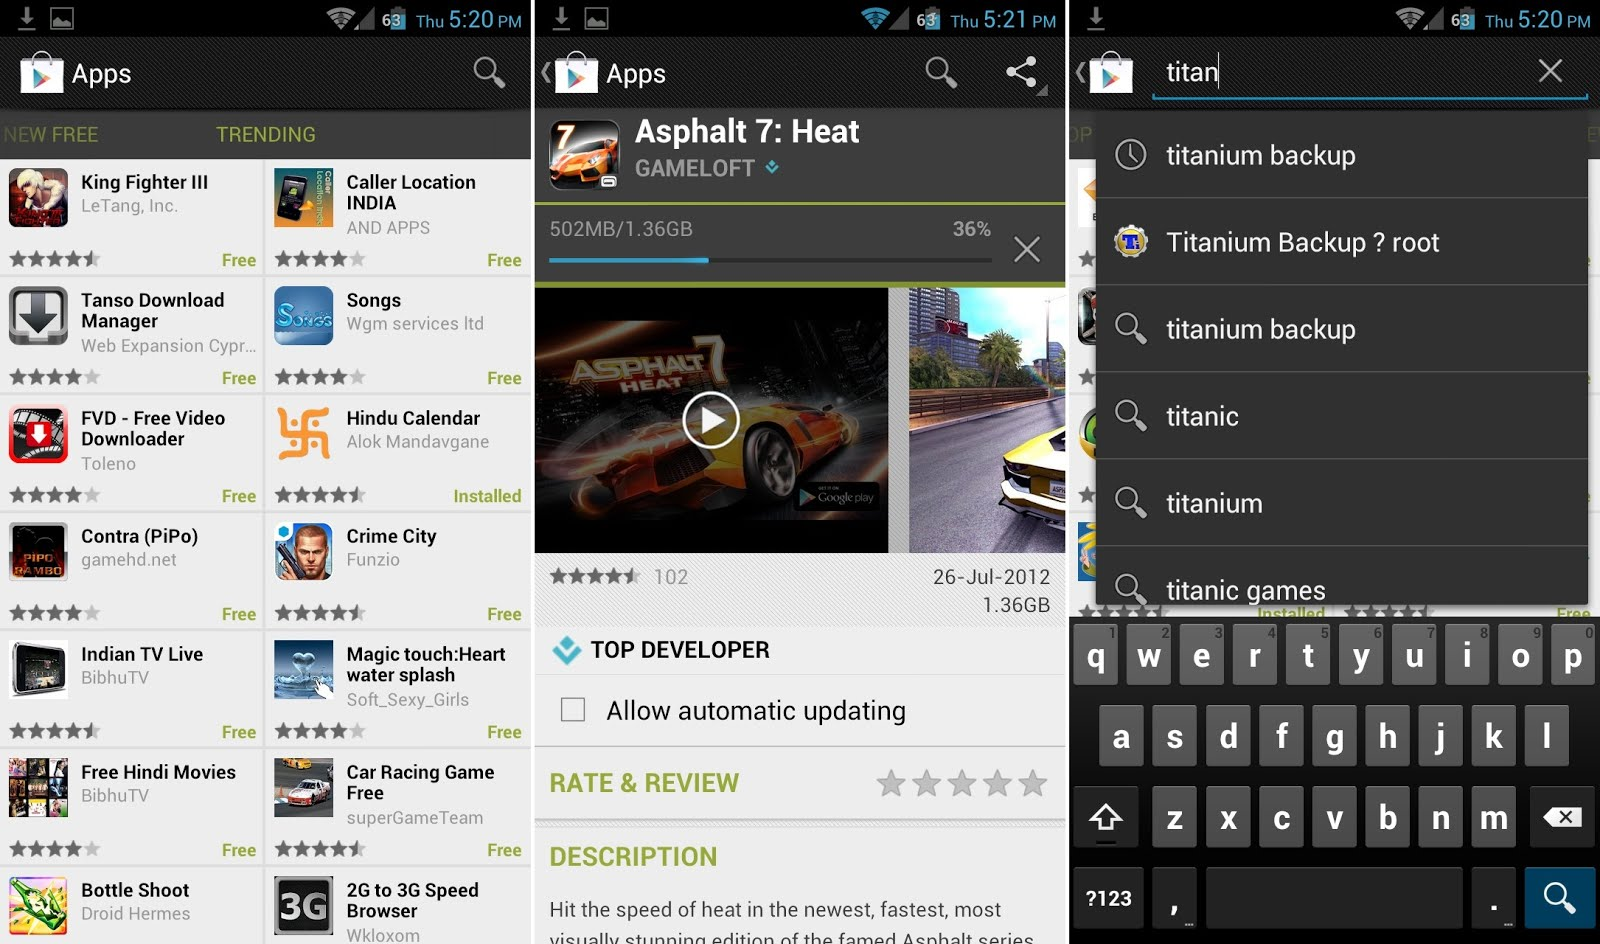
\includegraphics[scale=0.2]{images/Google-Play-Store-APK-3-7-15.jpg}
\caption{Google Play Store}
\end{figure}

{\bf App Store} is also a similar market application, but for apple products\ldots etc\ldots\\
\begin{figure}[H]
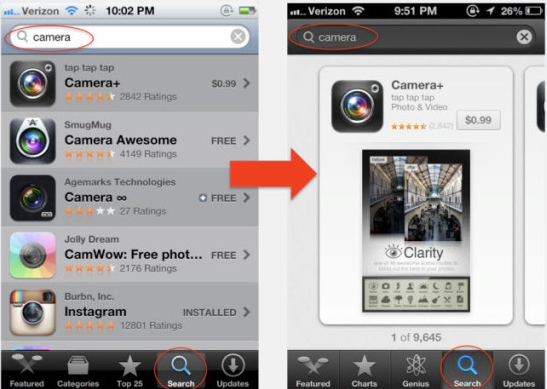
\includegraphics[scale=0.7]{images/png;base642dee0c596030bc1e.png}
\caption{App Store}
\end{figure}
These applications fit the assignment in the way that they are both market applications where one can download applications. This were useful for the development of the product, since it was possible to use the same principles in the assignment. It is also similar in the way that it is possible to browse for applications on the computer, and ''push'' the app to a mobile telephone. This, however, does not connect via bluetooth which the task assignment stated that the finished product should. Based on this, it was not possible to reuse the code or other parts of any of the applications in the development. 

\subsubsection{Over the air transfer}
Pebble is a watch that offers over the air transfer of applications. It is based on the same microchip as one of the newest Arduino\#, but contains an operating system written in C.
\begin{figure}[H]
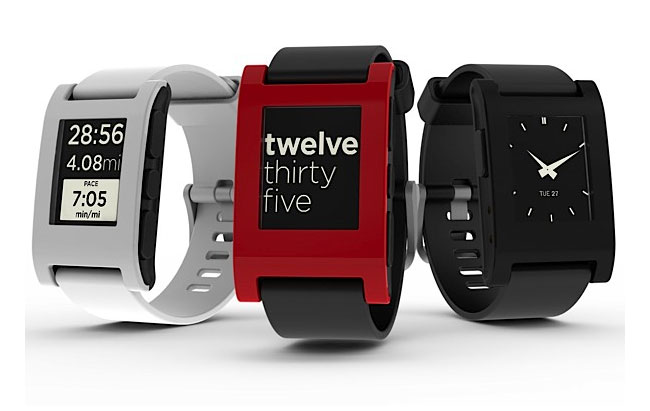
\includegraphics[scale=0.7]{images/Pebble-Smartphone-Watch.jpeg}
\caption{Pebble Watch}
\end{figure}
There is very little documentation on the Pebble website, so the potential reuse in this project appears minimal. %TODO Rename chapter to Reflection

\newpage
\addcontentsline{toc}{chapter}{Appendixes} %this line may break your compilation, and may require recompiation
\appendix
\chapter{Iterations}

This section contains an overview and a summary of each iteration of this project. The project was split into
iterations of two weeks, and the content is based on the activity plan and the status report that was delivered to the supervisor. In each iteration the use cases described in chapter ~\ref{usecases} is shown to present what the group was working on.

\section{Iteration 1}
Week 6 and 7
\subsection{Summary}
	These were the first two weeks of the project and the first group meeting was arranged.	Meeting with the customer to get the requirement specification and understanding of the projects goal was done.	Required libraries, licenses and other factors was taken in account before the group could start developing. No use cases were generated in this iteration, as basic research and planning had to be done before scenarios could be generated.
\subsection{Overview}
\begin{itemize}
	\item{Confirm understanding of the task}
	\item{Ideas for identifying the capabilities of an Arduino device and how to communicate these to the store client}
	\item{Investigate potential solutions to facilitate over the air installation of Arduino applications}
	\item{Start design the GUI for the Android application}
	\item{Research on Apache licenses}
	\item{Meeting with customer}
\end{itemize}

\section{Iteration 2}
Week 8 and 9
\subsection{Summary}
	Architectural work and design of the user interface of the Android application. Positive feedback on the GUI was received from the customer. Design of use cases and further research was performed.
\subsection{Overview}
\begin{itemize}
	\item{Think architectural}
	\item{Designing of GUI}
	\item{Research on over the air implementation}
	\item{Research Ubicollab libraries}
	\item{Use iJacket - generic application, Bluetooth connection code}
	\item{Implement a first sketch of the content provider}
	\item{Meeting with customer}
\end{itemize}

\section{Iteration 3}
Week 10 and 11
\subsection{Summary}
	Focus on Bluetooth connection and over the air implementation was prioritized these weeks. The application was taking form and the bugs were beginning to show up. Use cases 2, 3, 4 and 5 were in focus during this iteration. There were some issues with over the air because of incompatible licenses and much work was put into research. The Android application was estimated to be 50\% complete.

\subsection{Overview}
\begin{itemize}
	\item{Research Ubicollab libraries}
	\item{Finish design of the GUI}
	\item{Establish a Bluetooth connection between Android and Arduino}
	\item{Implement last draft of the content provider}
	\item{Meeting with customer}
\end{itemize}

\section{Iteration 4}\label{Iteration4}
Week 12 and 13
\subsection{Summary}
	This iteration became critical when it was discovered that existing implementations of the STK500 protocol were either incompatible with the required Apache v.2 license or not compatible with Android. An emergency meeting with the customer took place and it was decided to implement the STK500 protocol in Java. Developing the Sync Adapter was removed from the requirements, and the focus was moved to implementing the protocol as a library. Use cases 2, 3 and 4 were in focus during this iteration.

\subsection{Overview}
\begin{itemize}
	\item{Emergency meeting with customer}
	\begin{itemize}
		\item{Not possible to use existing solutions of STK500 protocol}
		\item{Agreement on implementing the STK500 in Java ourselves as a library}
	\end{itemize}
	\item{Research on STK500}
	\item{Unit test sketches}
	\item{Continued work on develop the Android application}
\end{itemize}

\section{Iteration 5}
Week 14 and 15
\subsection{Summary}
	Good progress and much was done. The group was more optimistic about the implementation of the protocol and the development of the application was almost complete.	The group was now split into two, where one group was writing the protocol, and the other group was writing Unit tests and polishing the last parts of the application. Use cases 4, 5 and 7 were in focus during this iteration.

\subsection{Overview}
\begin{itemize}
	\item{Added storage of hex-files to content provider}
	\item{Writing Robotium unit tests}
	\item{Writing the STK500 protocol in Java/Android}
	\item{Finishing the Android application except for the STK500 part}
	\item{Meeting with customer}
\end{itemize}

\section{Iteration 6}
Week 16 and 17

\subsection{Summary}
	Unexpected issues with programming the Arduino nearly caused the implementation to fail, requiring a meeting with the customer.
Suggestions for alternate solutions were presented, and it was decided to work in parallel on some of them. The customer was to attempt to ask some experts in the field for some code review.
Shortly after the meeting the problem was resolved.

\subsection{Overview}
\begin{itemize}
    \item{Meeting on protocol implementation problems}
    \item{Problem resolution}
	\item{Implement the STK500 to the Android application}
\end{itemize]

\section{Iteration 7}
Week 18 and 19

\subsection{Summary}
These were the last two weeks scheduled for the project. 

The final parts of the application were completed and the STK500 was implemented into the application as a library.
	A workshop with the customer at SINTEF was held, and an acceptance test and a usability test were performed. Most of the time was spent on completing the documentation.

\subsection{Overview}
\begin{itemize}
	\item{Workshop for SINTEF}
		\begin{itemize}
			\item{Demonstrate our finish application}
			\item{Acceptance testing}
			\item{Usability testing}
		\end{itemize}
\end{itemize}


\newpage
\listoftables
\listoffigures
\bibliographystyle{plain}
% We use MLA standard for citation. Create your citations at:
% \url{http://citationmachine.net/index2.php?reqstyleid=0&stylebox=1

% Remember to update the bibliography number as you add or remove bibitems.
\thispagestyle{plain}

\begin{thebibliography}{21}

	\bibitem{baudrate}{
		\emph{electronicdesign.com}
		N.P.. Web. 01 May 2013
		<\url{http://electronicdesign.com/communications/what-s-difference-between-bit-rate-and-baud-rate}>
	}

	\bibitem{kruchten}{
        Kroll, P., and P. Kruchten. \emph{The rational unified process made easy: A practitioner's guide to the rup}. Boston, MA: Addison-Wesley Professional, 2003. eBook.
    }

	\bibitem{scrum}{
		\emph{Scrum.org}.
		N.p.. Web. 13 Mar 2013
		<\url{http://www.scrum.org/Resources/What-is-Scrum}>.
		}

	\bibitem{sommerville}{
		Sommerville, Ian. \emph{Software Engineering}. 9th ed. Boston: Pearson Custom Publishing, 2011. Print.
	  	}

    \bibitem{poppendieck}{
        Poppendieck, M., and T. Poppendieck. \emph{Lean software development, an agile toolkit}. Addison-Wesley Professional, 2003. Print.
        }

    \bibitem{rn-42}{"Bluetooth Module - RN-42." Sparkfun.com. Sparkfun. Web. <https://www.sparkfun.com/products/10393>. 
    }

	\bibitem{hc-05}{"Bluetooth Module - HC-05." Iteadstudio.com. Itead Studio. Web. <ftp://imall.iteadstudio.com/Modules/IM120723009/DS_IM120723009.pdf>. 
    }

	\bibitem{testing-overview}{
		\emph{Microsoft.com}.
		N.p.. Web. 13 Mar 2013
		<\url{http://msdn.microsoft.com/en-us/library/aa292191(v=vs.71).aspx}>
	}

		\bibitem{unit-testing1}{
		\emph{Microsoft.com}.
		N.p.. Web. 13 Mar 2013
		<\url{http://msdn.microsoft.com/en-us/library/aa292197(v=vs.71).aspx}>
	}
	
	\bibitem{unit-testing2}{
		\emph{GeoSoft.no}.
		N.p.. Web. 13 Mar 2013
		<\url{http://geosoft.no/development/unittesting.html}>
	}

	\bibitem{unit-testing3}{
		\emph{Android.com}.
		N.p.. Web. 13 Mar 2013
		<\url{http://developer.android.com/tools/testing/testing\_android.html}>
	}

	\bibitem{Nielsen}{
		Nielsen, Jakob. ``Why you only need to test with 5 users.'' \emph{NNgroup.com}. N.p., 19 Mar 2000. Web. 16 Apr 2013. <\url{http://www.nngroup.com/articles/why-you-only-need-to-test-with-5-users/}>.
	}


    \bibitem{AVR068}{
        \emph{Atmel.com}.
        N.P.. Web. 8 Feb 2013
        <\url{http://www.atmel.com/Images/doc2591.pdf}>
    }
    
    \bibitem{StkBoot}{
		\emph{Google.com}
		N.P.. Web. 25 Mar 2013
		<\url{https://code.google.com/p/stkboot/}>
	}
	
	\bibitem{uOS-Embedded}{
		\emph{Google.com}
		N.P.. Web. 25 Mar 2013
		<\url{https://code.google.com/p/uos-embedded/}>
	}

    \bibitem{AVR061}{
        \emph{Atmel.com}.
        N.p.. Web. 26 Mar 2013
        <\url{http://www.atmel.com/Images/doc2525.pdf}>
    }
    	
	\bibitem{validation-testing}{
		\emph{Buzzle.com}.
		N.p.. Web. 13 Mar 2013
		<\url{http://www.buzzle.com/articles/validation-testing.html}>
	}
    	
    \bibitem{integration-testing2}{
		\emph{Microsoft.com}.
		N.p.. Web. 13 Mar 2013
		<\url{http://msdn.microsoft.com/en-us/library/aa292128(v=vs.71).aspx}>
	}
	
	\bibitem{functional-testing}{
		\emph{Wikipedia.org}.
		N.p.. Web. 13 Mar 2013
		<\url{http://en.wikipedia.org/wiki/Functional\_testing}>
	}

    \bibitem{android-dev-guide}{
    	\emph{Android.com}
    	N.p.. Web. 5 May 2013
    	<\url{http://developer.android.com/design}>
    }

    \bibitem{git-branch}{
    	\emph{http://git-scm.com/}
    	N.p.. Web. 12 May 2013
    	<\url{http://git-scm.com/book/en/Git-Branching-What-a-Branch-Is}>
    }

    \bibitem{websequencediagrams}{
    	\emph{http://www.websequencediagrams.com/}
    	N.p.. Web 12 May 2013
    	<\url{http://www.websequencediagrams.com/}>
    }
    
    \section*{Source of images}
    This section containts the all the sources for all the images used in the report. The images and sources that are not listed here is made by the project team. \\

    Figure~\ref{fig:sintef} in section~\ref{sec:sintef} : \\
    N.P.. Web. 19 Apr 2013\\
	<\url{http://www.sintef.no}> \\

	Figure~\ref{fig:ntnu} in section~\ref{sec:ntnu} : \\
	N.P.. Web. 19 Apr 2013\\
	<\url{http://www.ntnu.no}> \\

	Figure~\ref{fig:googleplay} in section~\ref{sec:googleplay} \\
	N.P.. Web. 13 Mar 2013\\
	<\url{http://droidtrends.com/wp-content/uploads/2012/07/Google-Play-Store-APK-3.7.15.jpg}> \\

	Figure~\ref{fig:pebblewatch} in section~\ref{sec:pebblewatch} : \\
	N.P.. Web. 19 Apr 2013\\
	<\url{http://getpebble.com/}> \\

	Figure~\ref{fig:SimpleArduinoWiring} in section~\ref{sec:SimpleArduinoWiring} : \\
	N.P.. Web. 19 Apr 2013\\
	<\url{http://fritzing.org/}> \\

	Figure~\ref{fig:rup} in section~\ref{sec:rup} \\
	N.P.. Web. 19 Apr 2013\\
	<\url{http://www.c3ns.com/c3nsservices_3.html}> \\
	
\end{thebibliography}


\end{document}
